\documentclass[a4paper,12pt]{article}

% Paquetes básicos
\usepackage[utf8]{inputenc}
\usepackage[T1]{fontenc}
\usepackage[spanish]{babel}
\usepackage{graphicx}
\usepackage{xcolor}
\usepackage{lipsum}
\usepackage{geometry}
\geometry{top=3cm, bottom=3cm, left=2.5cm, right=2.5cm}

% Paquetes para diseño
\usepackage{titlesec}
\usepackage{fancyhdr}
\usepackage{amsmath}
\usepackage{amssymb}
\usepackage{hyperref}
\usepackage{enumitem}
\usepackage{mathpazo}
\usepackage{amsmath}
\usepackage{amssymb}
\usepackage{mathpazo}
\usepackage{eulervm}
\usepackage{multicol}
\usepackage{float}
\usepackage{caption}
\usepackage{subcaption}
\usepackage{tcolorbox}

% Paquetes para el entorno lstlisting
\usepackage{listings}
\usepackage{inconsolata}

% Paquete para fondo
\usepackage{background}

% % Configuración de lstlisting
% \lstset{
%     language=Python,
%     basicstyle=\ttfamily\small,
%     keywordstyle=\color{blue}\bfseries,
%     stringstyle=\color{teal},
%     commentstyle=\color{gray}\itshape,
%     numbers=left,
%     numberstyle=\tiny\color{gray},
%     backgroundcolor=\color{black!5},
%     frame=single,
%     rulecolor=\color{black!50},
%     breaklines=true,
%     captionpos=b,
%     showstringspaces=false
% }

%COMANDOS
\newcommand{\betaEstimada}{\vec{\hat{\beta}}}
\newcommand{\ecuacion}[1]{\ensuremath{#1}}

% Configuración de título
\titleformat{\section}{\normalfont\Large\bfseries}{\thesection}{1em}{}

% Información del documento
\title{
    \vspace{-2cm}
    
\includegraphics[width=0.3\textwidth]{images/fccee.jpg} \\ % Cambia el logo si es necesario
    \LARGE Ingeniería Informática + ADE\\
    \large Universidad de Granada (UGR)\\[1cm]
}
\author{\textbf{Autor:} Ismael Sallami Moreno}
\date{\textbf{Asignatura:} Formulario y Resumen Econometría}


%encabezado y pie de página nivel profesional
\usepackage{fancyhdr}
\pagestyle{fancy}
\fancyhf{}
\fancyhead[L]{\leftmark}
\fancyhead[R]{\rightmark}
\fancyfoot[L]{\textbf{Ismael Sallami Moreno - GIIADE}}
\fancyfoot[C]{\thepage}
\fancyfoot[R]{\textbf{(UGR)} \today}
\renewcommand{\headrulewidth}{0.4pt}
\renewcommand{\footrulewidth}{0.4pt}
\setlength{\headheight}{15pt}
\setlength{\headsep}{10pt}
\setlength{\footskip}{20pt}
\usepackage{truncate}
\fancyhead[L]{\truncate{0.5\headwidth}{\leftmark}}
\fancyhead[R]{\truncate{0.5\headwidth}{\rightmark}}
\usepackage{mathpazo}
\usepackage{tcolorbox}

% Configuración del fondo
\backgroundsetup{
    scale=1,
    color=black,
    opacity=0.2,
    angle=0,
    position=current page.south,
    vshift=0pt,
    hshift=0pt,
    contents={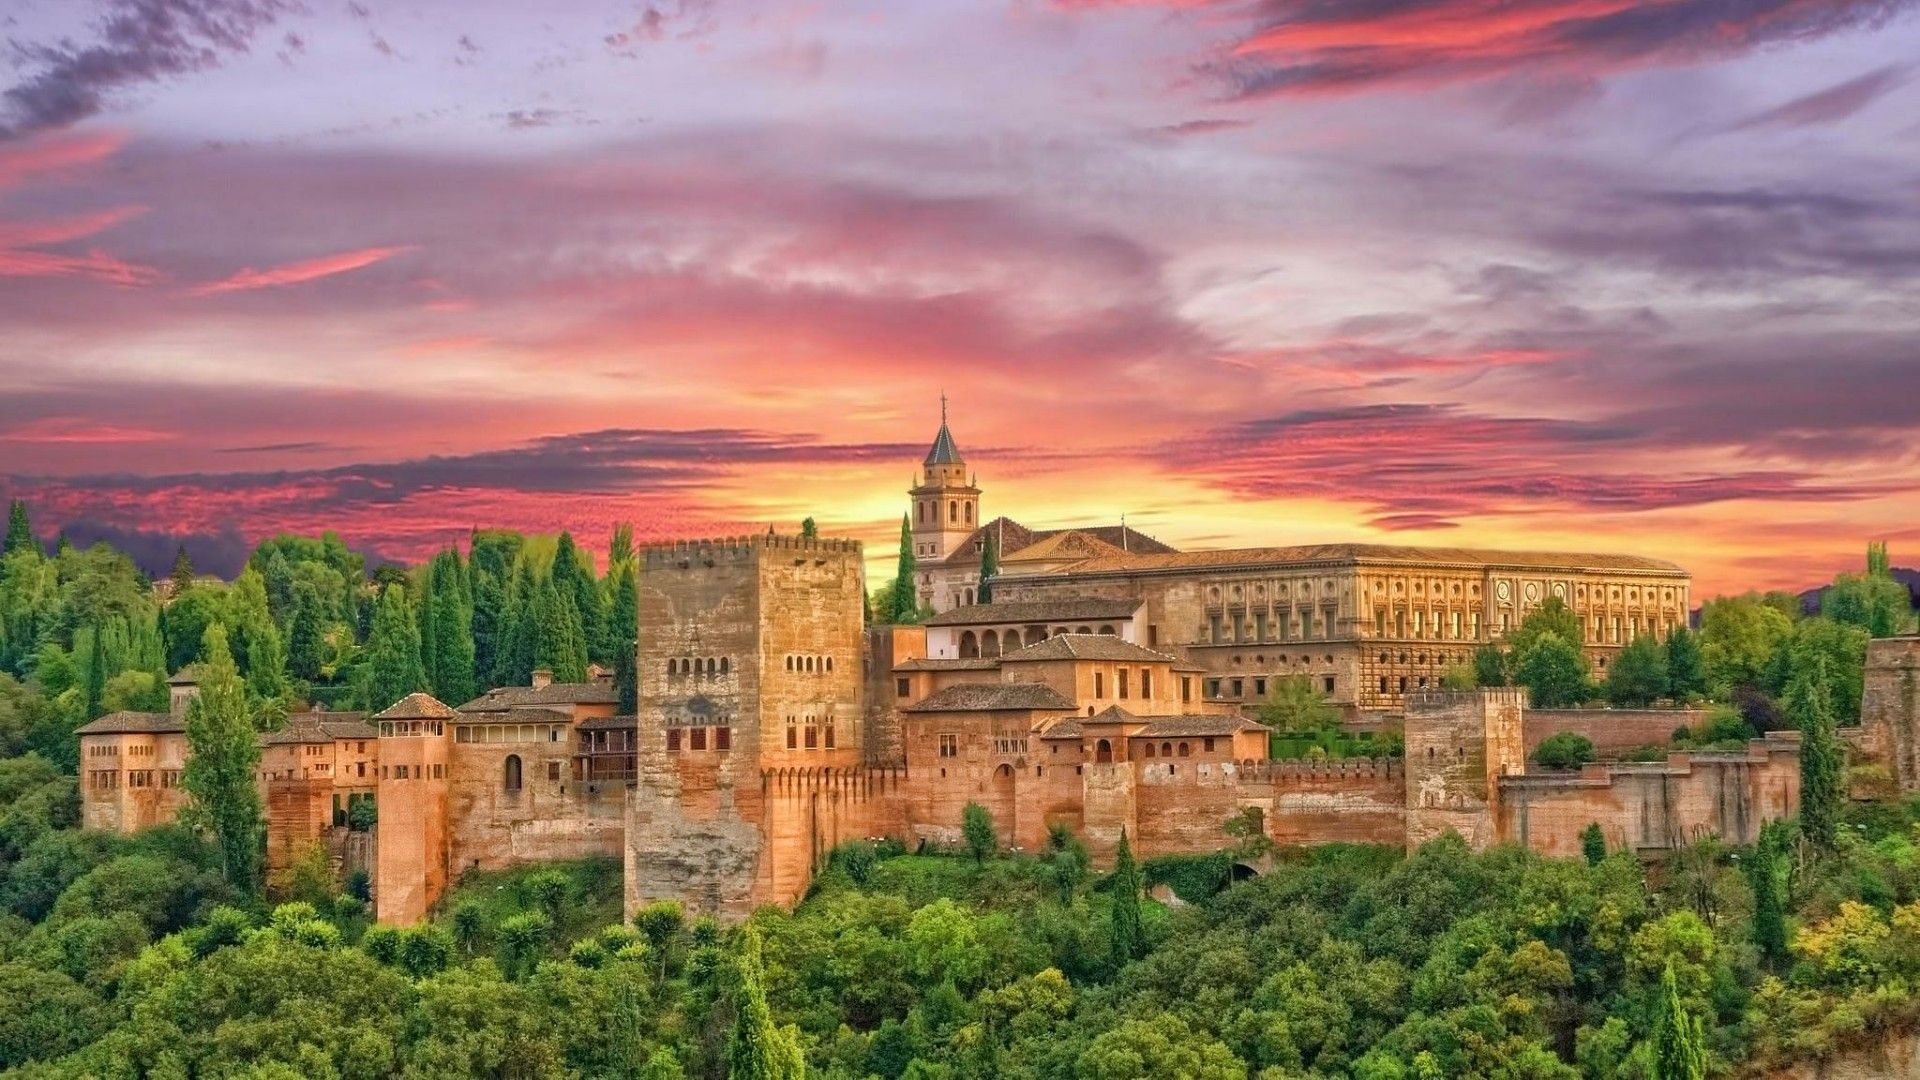
\includegraphics[width=\paperwidth,height=\paperheight,keepaspectratio]{images/granada.jpg}}
}

%lstlisting personalizado y completo para python
% Configuración de lstlisting
\lstset{
    inputencoding=utf8,          % Permite UTF-8
    extendedchars=true,          % Reconoce caracteres extendidos
    literate=                    % Configuración manual para tildes y símbolos
        {á}{{\'a}}1
        {é}{{\'e}}1
        {í}{{\'i}}1
        {ó}{{\'o}}1
        {ú}{{\'u}}1
        {ñ}{{\~n}}1
        {Á}{{\'A}}1
        {É}{{\'E}}1
        {Í}{{\'I}}1
        {Ó}{{\'O}}1
        {Ú}{{\'U}}1
        {Ñ}{{\~N}}1
        {¿}{{\textquestiondown}}1
        {¡}{{\textexclamdown}}1,
    basicstyle=\ttfamily,        % Fuente monoespaciada
    breaklines=true,             % Habilita salto de línea automático
    frame=single,                % Marco alrededor del código
    backgroundcolor=\color{gray!10}, % Fondo gris claro
    keywordstyle=\color{blue},   % Color para palabras clave
    commentstyle=\color{green},  % Color para comentarios
    stringstyle=\color{red}      % Color para strings
}
\lstdefinestyle{customcpp}{
    language=C++,                % Lenguaje de programación
    showspaces=false,            % No mostrar espacios
    showtabs=false,              % No mostrar tabulaciones
    tabsize=4,                   % Tamaño de tabulación
    showstringspaces=false,      % No mostrar espacios en strings
    numbers=left,                % Números de línea a la izquierda
    numberstyle=\tiny\color{gray}, % Estilo de los números de línea
    numbersep=5pt,               % Separación de los números de línea
    stepnumber=1,                % Mostrar número en cada línea
    basicstyle=\ttfamily\footnotesize, % Estilo básico del código
    keywordstyle=\bfseries\color{blue}, % Estilo de las palabras clave
    commentstyle=\itshape\color{green!50!black}, % Estilo de los comentarios
    stringstyle=\color{red},     % Estilo de los strings
    identifierstyle=\color{black}, % Estilo de los identificadores
    % procnamekeys={def,class},    % Palabras clave para nombres de funciones
    morekeywords={constexpr,nullptr,size_t}, % Más palabras clave
    emph={int,char,double,float,unsigned}, % Palabras a enfatizar
    emphstyle=\color{magenta},   % Estilo de las palabras enfatizadas
    backgroundcolor=\color{gray!10}, % Color de fondo
    frame=shadowbox,             % Marco con sombra
    rulesepcolor=\color{gray},   % Color de la línea de separación
    breakatwhitespace=false,     % No cortar en espacios en blanco
    breaklines=true,             % Cortar líneas largas
    captionpos=b,                % Posición del título (abajo)
    escapeinside={(*@}{@*)},     % Delimitadores para escapar a LaTeX
    morecomment=[l][\color{magenta}]{\#}, % Comentarios de una línea
    morecomment=[s][\color{orange}]{/*}{*/}, % Comentarios multilínea
    morestring=[b]",             % Strings entre comillas dobles
    morestring=[b]'              % Strings entre comillas simples
}
\lstdefinestyle{custompython}{
    language=Python,
    showspaces=false,
    showtabs=false,
    tabsize=4,
    showstringspaces=false,
    numbers=left,
    numberstyle=\tiny\color{gray},
    numbersep=5pt,
    stepnumber=1,
    basicstyle=\ttfamily\footnotesize,
    keywordstyle=\bfseries\color{blue},
    commentstyle=\itshape\color{green!50!black},
    stringstyle=\color{red},
    identifierstyle=\color{black},
    backgroundcolor=\color{gray!10},
    frame=shadowbox,
    rulesepcolor=\color{gray},
    breakatwhitespace=false,
    breaklines=true,
    captionpos=b,
    escapeinside={(*@}{@*)},
    morecomment=[l][\color{magenta}]{\#},
    morecomment=[s][\color{orange}]{/*}{*/},
    morestring=[b]",
    morestring=[b]'
}

% Inicio del documento
\begin{document}

% Portada
\maketitle
\thispagestyle{empty}

\begin{center}
    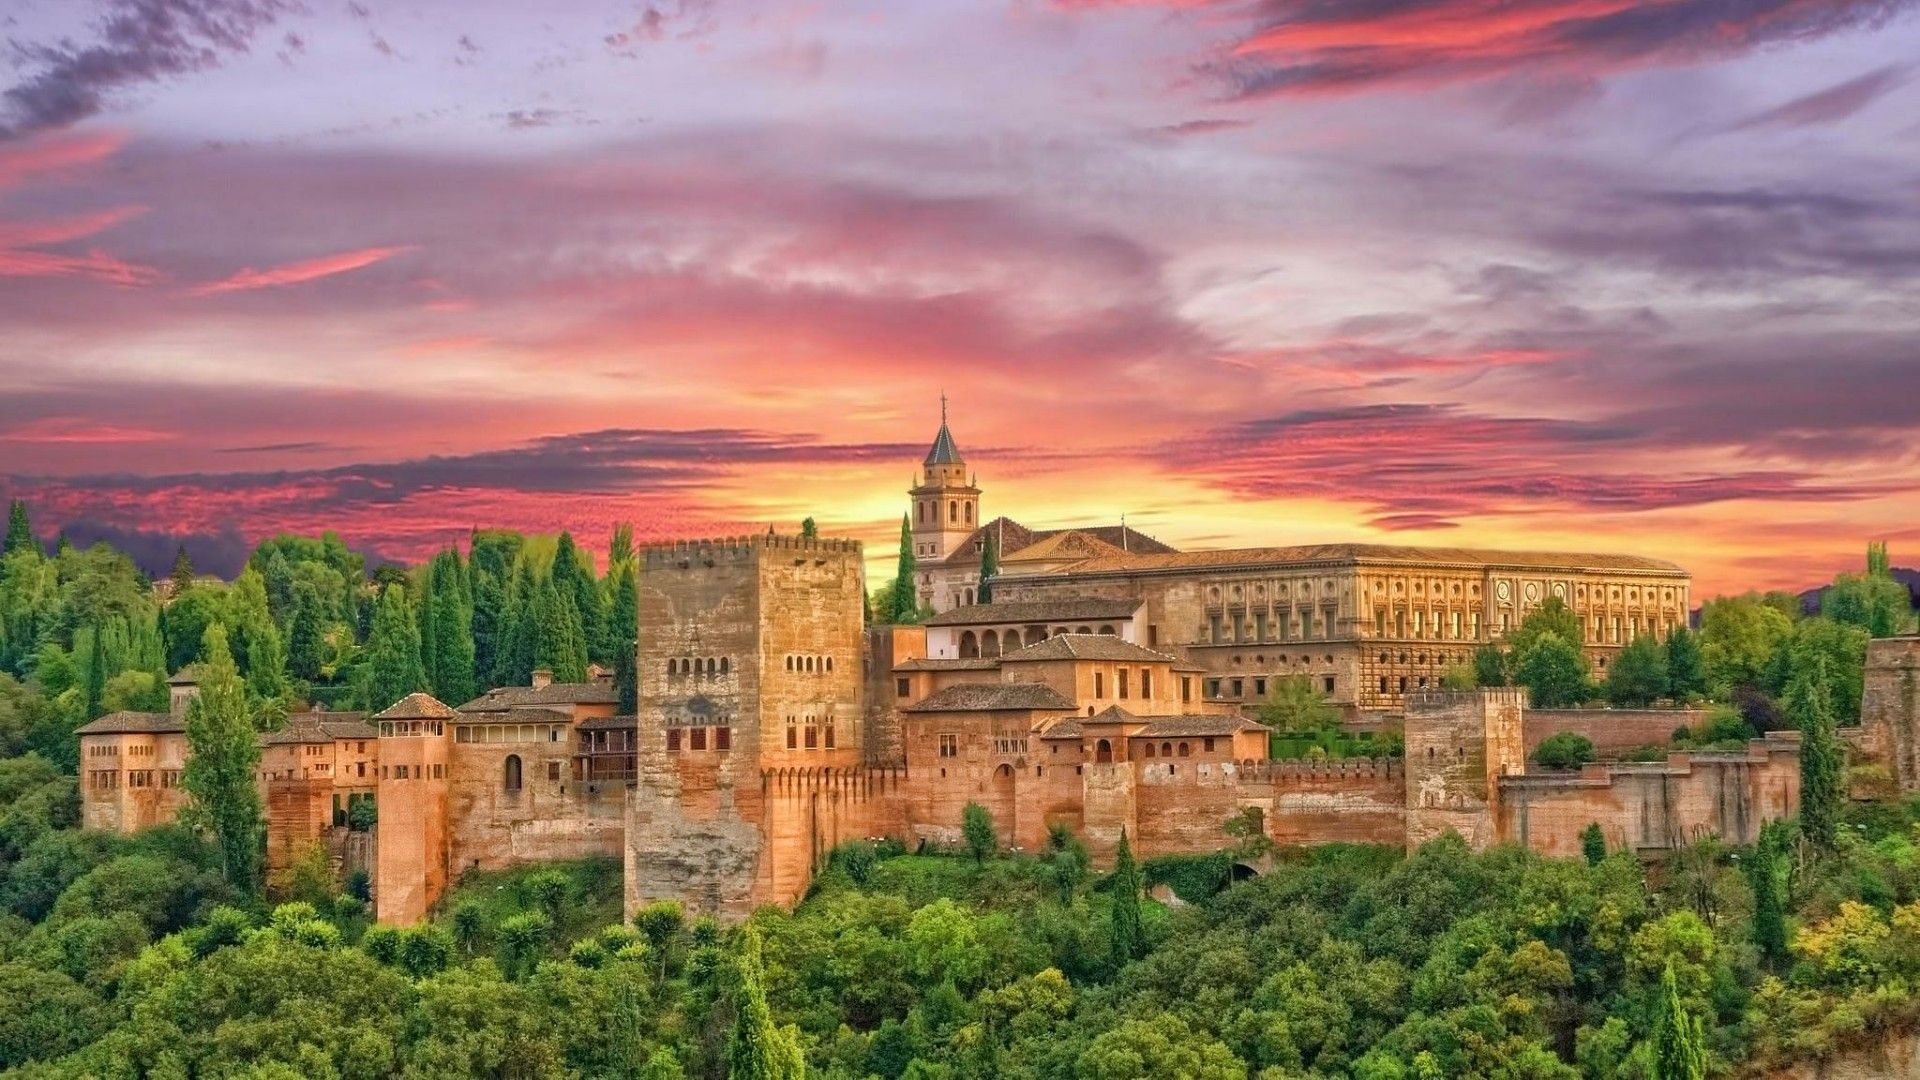
\includegraphics[width=\textwidth,height=0.4\textheight,keepaspectratio]{images/granada.jpg} \\ % Añade tu imagen de fondo
    \vfill
\end{center}

\newpage

% Índice (opcional)
\tableofcontents
\newpage

\section{Tema 2. Modelos de Regresión Lineal}

\subsection{Modelo Lineal Simple}

\begin{equation}
    Y_i \sim a + bx_i
\end{equation}

\subsection{Modelo Lineal Múltiple}

\begin{equation}
    Y_i = \beta_1 + \beta_2 x_{i2} + \beta_3 x_{i3} + \ldots + \beta_k x_{ik} + u_i
\end{equation}

\begin{itemize}
    \item El subíndice $i$ indica la observación.
    \item El subíndice $k$ indica el número de variables explicativas.
    \item El subíndice $u$ indica el término de error.
    \item Nota: $\beta_1$ es la constante, lleva asociado el valor 1 = $x_{i1}$ (por eso no se pone).
\end{itemize}

\subsection{Notación MLP}

\begin{equation}
    \vec{y} = \begin{pmatrix}
    Y_1 \\
    Y_2 \\
    \vdots \\
    Y_n
    \end{pmatrix}
    \end{equation}
    
    \begin{equation}
    X = \begin{pmatrix}
    1 & X_{21} & \cdots & X_{k1} \\
    1 & X_{22} & \cdots & X_{k2} \\
    \vdots & \vdots & \ddots & \vdots \\
    1 & X_{2n} & \cdots & X_{kn}
    \end{pmatrix}
    \end{equation}
    
    \begin{equation}
    \vec{\beta} = \begin{pmatrix}
    \beta_1 \\
    \beta_2 \\
    \vdots \\
    \beta_k
    \end{pmatrix}
    \end{equation}
    
    \begin{equation}
    \vec{u} = \begin{pmatrix}
    u_1 \\
    u_2 \\
    \vdots \\
    u_n
    \end{pmatrix}
    \end{equation}



\subsubsection{Notación Extra}

\subsubsection*{Matriz \ecuacion{X'X}}

\begin{equation}
    \begin{pmatrix}
        n & \sum_{i=0}^n X_{1i} & \cdots & \sum_{i=0}^n X_{ki} \\
        \sum_{i=0}^n X_{1i} & \sum_{i=0}^n X_{1i}^2 & \cdots & \sum_{i=0}^n X_{1i}X_{ki} \\
        \vdots & \vdots & \ddots & \vdots \\
        \sum_{i=0}^n X_{ki} & \sum_{i=0}^n X_{ki}X_{1i} & \cdots & \sum_{i=0}^n X_{ki}^2 \\
    \end{pmatrix}
\end{equation}

\subsubsection*{Matriz \ecuacion{X'Y}}

\begin{equation}
    \begin{pmatrix}
        \sum_{i=0}^n Y_{i} \\
        \sum_{i=0}^n X_{2i}Y_{i} \\
        \vdots \\
        \sum_{i=0}^n X_{ki}Y_{i} \\
    \end{pmatrix}
\end{equation}



\subsection{Supuestos}
\subsubsection{Linealidad}
\begin{equation}
    Y_i = \beta_1 + \beta_2 x_{i2} + \beta_3 x_{i3} + \ldots + \beta_k x_{ik} + u_i
\end{equation}

\subsubsection{Rango Completo Por Columnas}

\begin{equation}
    rango(X) = k
\end{equation}

\subsubsection{Exogeneidad}
\begin{equation}
    E(u_i|X_i) = 0
\end{equation}
\begin{itemize}
    \item El valor esperado de la esperanza que toman las variables explicativas es 0.
\end{itemize}

Por lo que si tenemos que: $Y_i = \vec{X_i^{t}}\vec{\beta}$, tenemos de forma inmediata que:
\begin{equation}
    E(Y_i|X_i) = \vec{X_i^{t}}\vec{\beta}
\end{equation}

\subsubsection{Causalidad}

\begin{itemize}
    \item Relación de causalidad es unidireccional.
    \item Las variables aparecen en el lado derecho de la ecuación, pero no al contrario.
    \item La variable dependiente $Y_i$ adoptará un carácter aleatorio.
\end{itemize}

\subsubsection{Perturbación}
\begin{itemize}
    \item Esta centrada, es decir, $E(u_i) = 0 \forall i=1,2,\ldots,n$
    \item Es homocedástica, es decir, $Var(u_i) = E[u_i^{2}]= \sigma^2 \forall i=1,2,\ldots,n$
    \item Si es incorrelada implica que $cov[u_iu_j] = E[u_iu_j]=0$. Cuando es $\neq$ 0 decimos que hay un problema de autocorrelación.
\end{itemize}

Como consecuencia tenemos que:
\begin{equation}
    var[\vec{u}] = E[(\vec{u}-E[\vec{u}])(\vec{u}-E[\vec{u}])^{t}] = E[\vec{u}\vec{u}^{t}]
\end{equation}
Para la demostración de esta operación pincha \href{https://github.com/ElblogdeIsmael/ElblogdeIsmael.github.io/blob/main/Asignaturas/Tercer%20A%C3%B1o/ECO/Formulario/FCCEE/ecotema2_1.pdf}{aquí} para verla.

\subsubsection{Normalidad de la perturbación}

Se considera que la perturbación aleatoria $u_i$ se distribuye normalmente con media 0 y varianza $\sigma^2$, es decir, $u_i \sim N(0,\sigma^2)\forall i=1,\ldots,n$.\\

En este caso supondremos que $\vec{u}$ se distribuye normalmente, es decir, $\vec{u} \sim N(\vec{0},\sigma^2I_n)$\footnote{distribución normal multivariante con vector de medias nulo y matriz de varianzas-covarianzas $\sigma^2I_n$}.

\subsection{Estimación Míminos Cuadrados Ordinarios (MCO)}

Para estimar los parámetros $\beta$ utilizaremos el MCO, denotando a $\hat{\vec{y}}$ el valor ajustado de $\vec{y}$, es decir, $\hat{\vec{y}} = X\hat{\vec{\beta}}$. \\

En este caso el valor de los residuos se obtiene como:
\begin{equation}
    \vec{e}=\vec{y}-\hat{\vec{y}} = \vec{y}-X\hat{\vec{\beta}}
\end{equation}

Debemos de minimizar la suma de los cuadrados de los residuos:

\begin{equation}
    \min_{\vec{\beta}} \sum_{i=1}^{n} e_i^2
\end{equation}

Tendremos como función a minimizar: $f(\hat{\vec{\beta}})=\vec{e}^{\,\,t}  \vec{e}$

\subsubsection{Pasos a seguir}
\begin{enumerate}
    \item Definimos la expresión a minimizar. Se debe de definir la suma de los cuadrados de los residuos:
    \begin{equation}
        f(\vec{\hat{\beta}}) = (\vec{y} - X\vec{\hat{\beta}})^{t}(\vec{y} - X\vec{\hat{\beta}})
    \end{equation}
    \item Derivamos con respecto a $\vec{\hat{\beta}}$ e igualamos a 0:
    \begin{equation}
        \frac{\partial f(\vec{\hat{\beta}})}{\partial \vec{\hat{\beta}}} = 0
    \end{equation}
    \item Despejamos el vector de parámetros, debemos de considerar el supuesto del rango completo por columnas, verificándose que $\rho (X^tX) = 1$, condición necesaria para que exista $(X^tX)^{-1}$
    \item Para que la solución sea mínimo se ha de cumplir:
    \begin{equation}
        \text{Hess}(f) = 2X^tX > 0 \text{ and } 
        (A>0 \text{ si } z^tAz > 0 \,\,\forall z \neq 0)
    \end{equation}
\end{enumerate}

% Si el modelo tiene término independiente entonces se tiene
\subsubsection*{Si el modelo tiene término independiente entonces se tiene}
$\vec{\beta} = \left( \begin{array}{cccc}
    n & \sum_{i=1}^{n} X_{2i} & \cdots & \sum_{i=1}^{n} X_{ki} \\
    \sum_{i=1}^{n} X_{2i} & \sum_{i=1}^{n} X_{2i}^2 & \cdots & \sum_{i=1}^{n} X_{2i}X_{ki} \\
    \vdots & \vdots & \ddots & \vdots \\
    \sum_{i=1}^{n} X_{ki} & \sum_{i=1}^{n} X_{ki}X_{2i} & \cdots & \sum_{i=1}^{n} X_{ki}^2 \\
    \end{array} \right)^{-1}
    \left( \begin{array}{c}
    \sum_{i=1}^{n} Y_{i} \\
    \sum_{i=1}^{n} X_{2i}Y_{i} \\
    \vdots \\
    \sum_{i=1}^{n} X_{ki}Y_{i} \\
\end{array} \right)$
    
    % En el caso de que el modelo carezca del término independiente entonces:
    \subsubsection*{En el caso de que el modelo carezca del término independiente entonces:}
    $\vec{\beta} = \left( \begin{array}{cccc}
    \sum_{i=1}^{n} X_{1i}^2 & \sum_{i=1}^{n} X_{1i}X_{2i} & \cdots & \sum_{i=1}^{n} X_{1i}X_{ki} \\
    \sum_{i=1}^{n} X_{2i}X_{1i} & \sum_{i=1}^{n} X_{2i}^2 & \cdots & \sum_{i=1}^{n} X_{2i}X_{ki} \\
    \vdots & \vdots & \ddots & \vdots \\
    \sum_{i=1}^{n} X_{ki}X_{1i} & \sum_{i=1}^{n} X_{ki}X_{2i} & \cdots & \sum_{i=1}^{n} X_{ki}^2 \\
    \end{array} \right)^{-1}
    \left( \begin{array}{c}
    \sum_{i=1}^{n} X_{1i}Y_{i} \\
    \sum_{i=1}^{n} X_{2i}Y_{i} \\
    \vdots \\
    \sum_{i=1}^{n} X_{ki}Y_{i} \\
\end{array} \right)$
    
\subsection{Estimación Míminos Cuadrados Ordinarios Restringidos(MCO(R))}

\begin{equation}
    \widehat{\beta_R} = \widehat{\beta} - (R(X'X)^{-1})^t \times [R(X'X)^{-1}R']^{-1} \times R\widehat{\beta}
\end{equation}

\subsection{Propiedades Algebraicas de los MCO}

\subsubsection*{Considerando que SI hay ti}

\begin{itemize}
    \item Las variables exógenas son ortogonales al vector de los residuos: $X^t\vec{e}=\vec{0}$
    \subsubsection*{Demostración}
    \begin{enumerate}
        \item Tenemos que $-2X^t\vec{y} + 2X^tX\betaEstimada = \vec{0}$
        \item Si operamos nos queda que $X^t(\vec{y}- X\betaEstimada) = \vec{0}$
        \item Aplicando que $\vec{\hat{y}} = X\betaEstimada$
        \item Queda demostrado que $X^t\vec{e}=\vec{0}$
    \end{enumerate}
    \item La suma de los residuos mínimos cuadráticos es 0: $\sum_{i=1}^{n} e_i = 0$
    \item La suma de los valores observados coincide con la suma de los valores estimados: $\sum_{i=1}^{n} y_i = \sum_{i=1}^{n} \hat{y}_i$
    \item Suma Cuadrados 
    \begin{itemize}
        \item $SCT = \sum_{i=1}^{n} (y_i - \bar{y})^2 = \vec{y}^{\,\,t} \vec{y} - n \cdot \bar{Y}^2$
        \item $SCR = \sum_{i=1}^{n} (y_i - \hat{y}_i)^2 = \vec{y}^{\,\,t}  \vec{y} - \vec{\beta}^t \vec{X}^t \vec{y}$
        \item $SCE = \sum_{i=1}^{n} (\hat{y}_i - \bar{y})^2 = \vec{\beta}^t\footnote{En la práctica la simbología de t = traspuesta = \textit{prima = '}} \vec{X}^t \vec{y} - n \cdot \bar{Y}^2$
    \end{itemize}
    \item  SCT = SCR + SCE
    \item \ecuacion{\vec{\hat{y}}\vec{e}=0}
    % % Explicación de la ecuación
    % \noindent
    % La ecuación \(\vec{\hat{y}}\vec{e}=0\) representa un producto vectorial entre dos vectores, \(\vec{\hat{y}}\) y \(\vec{e}\), que resulta en el vector nulo. En esta ecuación:
    % \begin{itemize}
    %     \item \(\vec{\hat{y}}\) es un vector unitario en la dirección \(y\).
    %     \item \(\vec{e}\) es otro vector en el espacio.
    %     \item El producto vectorial \(\vec{\hat{y}} \times \vec{e}\) da como resultado el vector nulo \(\vec{0}\), lo que implica que los vectores \(\vec{\hat{y}}\) y \(\vec{e}\) son paralelos o uno de ellos es el vector nulo.
    % \end{itemize}
\end{itemize}


\subsection{Bondad del Ajuste}

\begin{equation}
    R^2 = \frac{SCE}{SCT} = \frac{\sum_{i=1}^n(\hat{Y}-\bar{Y})^2}{\sum_{i=1}^n(Y_i-\bar{Y})^2}
\end{equation}

\subsubsection*{NOTA IMPORTANTE:}
Si el modelo tiene término independiente entonces $R^2$ se puede expresar como:
\begin{equation}
    R^2 = 1 - \frac{SCR}{SCT}
\end{equation}

\subsection{Bondad del Ajuste Corregido}

\begin{equation}
    \bar{R^2} = 1- \frac{SCR/(n-k)}{SCT/n-1} = 1-(1-R^2) * \frac{n-1}{n-k}
\end{equation}


\subsection{Criterio de Akaike}
\begin{equation}
    AIC = ln(\frac{SCR}{n}) + \frac{2k}{n}
\end{equation}

\subsection{Criterio de Schwarz}
\begin{equation}
    BIC = ln(\frac{SCR}{n}) + \frac{kln(n)}{n}
\end{equation}

\section{Tema 3: Estimación y Contraste de Hipótesis}


\subsection{Valor Esperado y Varianza de los EMCO (Estimadores mínimos cuadrados ordinarios)}

\subsubsection{Valor Esperado de los EMCO}
\begin{enumerate}
    \item El estimador de \ecuacion{\vec{\beta}} del modelo \ecuacion{\vec{y}=X\vec{\beta}+\vec{u}} es: 
    \[
        \hat{\vec{\beta}} = (X^tX)^{-1}X^t\vec{y}
    \]
    \item Si en esta sustituimos \ecuacion{\vec{y} = X\vec{\beta}+\vec{u}} nos quedaría:
    \[
        \hat{\vec{\beta}} = (X^tX)^{-1}X^t(X\vec{\beta}+\vec{u}) = \vec{\beta} + (X^tX)^{-1}X^t\vec{u}
    \]
    \item Por lo que E[\ecuacion{\hat{\vec{\beta}}}] = \ecuacion{\vec{\beta}}
    \begin{itemize}
        \item Debido a que E[\ecuacion{\vec{u}}] = \ecuacion{\vec{0}} \ecuacion{\rightarrow} \textbf{\ecuacion{\vec{\hat{B}}} es un estimador insesgado de \ecuacion{\vec{\beta}}}
    \end{itemize}
\end{enumerate}

\subsubsection{Varianza de los EMCO}

\begin{enumerate}
    \item \(\text{var}(\hat{\vec{\beta}}) = \sigma^2(X^tX)^{-1}\)
    Para ello debemos de seguir estos pasos:   
    \begin{enumerate}
        \item La varianza es igual a:
        \[
            \text{var}(\hat{\vec{\beta}}) = E[(\hat{\vec{\beta}}-E[\hat{\beta}]) (\hat{\vec{\beta}}-E[\hat{\beta}])^{t}]
        \]
        \item Si en la ecuación anterior sustituiimos \ecuacion{\hat{\vec{\beta}} = \vec{\beta} + (X^tX)^{-1}X^t\vec{u}} nos queda:
        \[
            \text{var}(\hat{\vec{\beta}}) = E[((X^tX)^{-1}X^t\vec{u})((X^tX)^{-1}X^t\vec{u})^{t}]
        \]
        \item Acto seguido, debemos de aplicar la propiedad de las matrices de \ecuacion{(AB)^t = B^tA^t}:
        \[
            \text{var}(\hat{\vec{\beta}}) = E[(X^tX)^{-1}X^t\vec{u}\vec{u}^tX(X^tX)^{-1}]
        \]
        \item Si aplicamos la propiedad de la esperanza de un producto de matrices \ecuacion{E[AB] = E[A]E[B]}:
        \[
            \text{var}(\hat{\vec{\beta}}) = (X^tX)^{-1}X^tE[\vec{u}\vec{u}^t]X(X^tX)^{-1}
        \]
        \item Si aplicamos la propiedad de la varianza de un vector \ecuacion{E[\vec{u}\vec{u}^t] = \sigma^2I_n}:
        \[
            \text{var}(\hat{\vec{\beta}}) = \sigma^2(X^tX)^{-1}X^tX(X^tX)^{-1} = \sigma^2(X^tX)^{-1}
        \]
        \item Con esto quedaría demostrado que \ecuacion{\text{var}(\hat{\vec{\beta}}) = \sigma^2(X^tX)^{-1}}
    \end{enumerate}
\end{enumerate}


\subsection{Teorema de Gauss-Markov}

Según este teorema tenemos que los estimadores de los mínimos cuadrados ordinarios son:
\begin{itemize}
    \item óptimos
    \item lineales
    \item insesgados    
\end{itemize}

\subsubsection*{Nota:}
Podemos decir que de todos los estimadores de \ecuacion{\vec{\beta}}, el EMCO es el que presenta \textit{ menor matriz de varianzas-covarianzas}.

\subsubsection{Demos}
\begin{itemize}
    \item \textbf{Demo I}: \ecuacion{\betaEstimada} es lineal con respecto a \ecuacion{\vec{y}}
    \subsubsection*{Demostración}
    \begin{enumerate}
        \item si definimos una matriz de dimensiones k*n \ecuacion{W = (X^tX)^{-1}X^t}
        \item es fácil demostrar que que \ecuacion{\vec{B} = W\vec{y}} ya que \ecuacion{\vec{B} = (X^tX)^{-1}X^t\vec{y}}
    \end{enumerate}
    \item \textbf{Demo II}: \ecuacion{\betaEstimada} es insesgado de \ecuacion{\vec{\beta}}\footnote{Queda demostrado anteriormente ya que se verificaba que la esperanza del parámetro a estimar era igual al parámetro.}
    \item  \textbf{Demo III}: \ecuacion{\betaEstimada} es un estimador óptimo de \ecuacion{\vec{\beta}}
    \subsubsection*{Demostración}
    \subsubsection*{- Esperanza}
    Para la demostración debemos de seguir los siguientes pasos:
    \begin{enumerate}
        \item Suponemos un estimador alternativo \ecuacion{\vec{\hat{\beta}}^*}
        \item Como se cumple que es lineal respecto de \ecuacion{\vec{\beta}}, entonces tenemos que \ecuacion{\vec{\hat{\beta}}^* = C\vec{y}}, es decir, existe un C que cumple la anterior condición de dimensiones k*n
        \item Además ha de ser insesgado, por lo que tenemos que \ecuacion{E[\vec{\hat{\beta}}^*] = \vec{\beta}}
        \item Si seguimos resolviendo tenemos que:
        \[
            E[\vec{\hat{\beta}}^*] = E[C\vec{y}]
        \]
        \item Aplicamos que \ecuacion{\vec{y} = X\vec{\beta}+\vec{u}}:
        \[
            E[C\vec{y}] = E[C(X\vec{\beta}+\vec{u})] = E[CX\vec{\beta}+C\vec{u}] = CX\vec{\beta}+CE[\vec{u}]
        \]
        \item Como sabemos que \ecuacion{E[\vec{u}] = 0}, nos queda:
        \[
            CX\vec{\beta}+CE[\vec{u}] = CX\vec{\beta}
        \]
        \item Volvemos al tema de insesgadez, para que sea insesgado (que se debe de cumplir en este punto) debe de que \ecuacion{CX=I_k}
        \item Por lo que tenemos de nuevo nuestro estimador anterior, podemos concluir la demostración afirmando que \ecuacion{\betaEstimada} es un estimador óptimo de \ecuacion{\vec{\beta}}
    \end{enumerate}
    \subsubsection*{- Varianza}
    \begin{itemize}
        \item Si la calulamos de igual manera a la anterior y usando la matriz C y aplicando que $E[(\widehat{\beta^*}^t)- E[\widehat{\beta^*}^t]] = C\vec{u}$, nos queda que:
        \[
            = E[C\vec{u}*\vec{u}^tC^t] = C\sigma^2I_nC^t = \sigma^2CC^t \footnote{Hemos usado que \ecuacion{E[\vec{u}\vec{u}^t] = \sigma^2I_n}}
        \] 
        \item  Sabiendo que \ecuacion{\betaEstimada = W\vec{y}} y \ecuacion{\betaEstimada^* = C\vec{y}}
        \item Denotamos D = C-W
        \item Tenemos que:
        \[
            DX = (C-W)X = CX-WX = CX - (X^tX)^{-1}X^tX = I_k - I_k = 0_k
        \]
        \item podemos afirmar además, que en base a lo definido anteriormente:
        \[
            \text{var}(\betaEstimada^*) = \sigma^2CC^t = \sigma^2(W+D)\footnote{Usamos que \ecuacion{C = W+D}}(W+D)^t = \sigma^2(WW^t + WD^t + DW^t + DD^t)\footnote{De la anterior forma también es válida esta es más extensa, esta sirve para comparar las varianzas como vamos a ver a continuación}
        \]
        \subsubsection*{Comparación de varianzas}
        \begin{itemize}
            \item \ecuacion{WW^t = ((X^tX)^{-1}X^t)((X^tX)^{-1}X^t)^t = (X^tX)^{-1}X^tX(X^tX)^{-1} = (X^tX)^{-1}}
            \item \ecuacion{WD^t = ((X^tX)^{-1}X^t)(D)^t = (X^tX)^{-1}X^t(C-W)^t = (X^tX)^{-1}X^t(C^t-W^t) = (X^tX)^{-1}X^tC^t - (X^tX)^{-1}X^tW^t = 0}
            \item \ecuacion{DW^t = D((X^tX)^{-1}X^t)^t = 0}
        \end{itemize}
        \item Aplicando esto nos queda que:
        \[
            \ecuacion{\text{var}(\vec{\hat{\beta}}^*) = \sigma^2DD^t + \text{var}(\vec{\hat{\beta}})}
        \]
        \item Como sabemos el primer término es siempre positivo, por lo que podemos afirmar que:
        \[
            \ecuacion{\text{var}(\vec{\hat{\beta}}^*) - \text{var}(\vec{\hat{\beta}}) = \sigma^2DD^t \geq 0 \rightarrow \text{var}(\vec{\hat{\beta}}^*) \geq \text{var}(\vec{\hat{\beta}})}
        \]
        \item Vemos que la  varianza también es mayor, por lo que podemos concluir que \ecuacion{\vec{\hat{\beta}}^*} es un estimador peor que \ecuacion{\vec{\hat{\beta}}}
    \end{itemize}

\end{itemize}

\subsection{Estimación de \ecuacion{\sigma_u^2}}

Sabemos que el vector de los residuos es;
\[
    \vec{e} = \vec{y} - \hat{\vec{y}} = \vec{y} - X\hat{\vec{\beta}}
\]

Si desarrollamos nos queda que:

\[
    (I_n - X(X^tX)^{-1}X^t)\vec{y} = M_x\vec{y}
\]

Para ello debemos de aplicar que:
\[
\hat{\vec{y}} = X\hat{\vec{\beta}} = X(X^tX)^{-1}X^t\vec{y}
\]

Y sacar factor común \ecuacion{\vec{y}}. \\\\

La matriz \ecuacion{M_x} se conoce como la matriz complemento del proyector ortogonal, cuyas propiedades son:
\begin{itemize}
    \item simétrica\footnote{Una matriz es simétrica si es igual a su traspuesta \ecuacion{A = A^t}}
    \item idempotente\footnote{Una matriz es idempotente si al elevarla al cuadrado nos da la misma matriz \ecuacion{A^2 = A}}
    \item traza(\ecuacion{M_x}) = n - k
    \item \ecuacion{M_xX} = X - X = 0   
\end{itemize} 

Si sustituimos \ecuacion{\vec{y} = X\vec{\beta} + \vec{u}} en la ecuación anterior nos queda que:
\[
    \vec{y} = M_x\vec{y} = M_xX\vec{\beta} + M_x\vec{u} = M_x\vec{u}\footnote{Ya que \ecuacion{M_xX = 0}}
\]

Si tomamos valores esperados obtenemos que (\ecuacion{E[\vec{e^t}\vec{e}] = }):
\begin{enumerate}
    \item \ecuacion{E[(M_x\vec{u})^t(M_x\vec{u})] }
    \item = \ecuacion{E[\vec{u}^tM_x\vec{u}]}\footnote{Ya que \ecuacion{M_x} es simétrica e idempotente}
    \item = \ecuacion{E[\text{traza}(\vec{u^t}M_x\vec{u})]}
    \item = \ecuacion{\text{traza}(M_xE[\vec{u^t}\vec{u}])}
    \item = \ecuacion{\text{traza}(\sigma^2M_x)}
    \item = \ecuacion{\sigma^2\text{traza}(M_x)}
    \item = \ecuacion{\sigma^2(n-k)}
\end{enumerate}

Finalmente, nos queda que \ecuacion{E[\vec{e^t}\vec{e}] = \sigma^2(n-k)}, por lo que como \ecuacion{E[\frac{\vec{e^t}\vec{e}}{n - k}] = \sigma^2} podemos afirmar que \ecuacion{\hat{\sigma}^2 = \frac{\vec{e^t}\vec{e}}{n - k} = \frac{SCR}{n-k}} es un estimador insesgado de \ecuacion{\sigma_u^2}


\subsection{Estimación de la varianza de los EMCO}

Como sabemos la varianza del EMCO \ecuacion{\vec{\beta}} es \ecuacion{\sigma^2(X^tX)^{-1}}, por lo que depende de la varianza de la perturbación y como sabemos el estimador de la varianza de la perturbación es: \ecuacion{\hat{\sigma}^2 = \frac{SCR}{n-k}}.\\

Por lo que nos queda que la varianza del EMCO es:
\begin{equation}
    \text{var}(\vec{\hat{\beta}}) = \frac{SCR}{n-k} * (X^tX)^{-1}
\end{equation}

\subsection{Supuesto de Normalidad e Inferencia}

\textbf{Supuesto de normalidad:} Supongamos que \( \vec{u} \sim N(\vec{0}, \sigma^2 I_n) \).

\textbf{Propiedades del estimador}: 
\begin{itemize}
    \item Dado que \( \vec{\hat{\beta}} = \vec{\beta} + (X^t X)^{-1} X^t \vec{u} \), por el Teorema de Gauss-Markov, se tiene que:
    \[ \vec{\hat{\beta}} \sim N(E[\vec{\hat{\beta}}], \text{var}(\vec{\hat{\beta}})) = N(\vec{\beta}, \sigma^2 (X^t X)^{-1}). \]

    \item Equivalentemente, se cumple:
    \[ (\vec{\hat{\beta}} - \vec{\beta}) \sim N(\vec{0}, \sigma^2 (X^t X)^{-1}). \]

\end{itemize}

\textbf{Distribución del residuo:}
\begin{itemize}
    \item Como se verifica que \( \vec{e}^{\,\,t} \vec{e} = \vec{u}^t M_X \vec{u} \), y dado que \( \vec{u} \sim N(\vec{0}, \sigma^2 I_n) \), y que \( M_X \) es simétrica, idempotente y tiene rango \( \rho(M_X) = n - k \), concluimos que:
    \[ \frac{1}{\sigma^2} \vec{u}^t M_X \vec{u} \sim \chi^2_{n-k}. \]

    \item Por tanto, se tiene que:
    \[ \frac{(n-k) \hat{\sigma}^2}{\sigma^2} \sim \chi^2_{n-k}. \]
\end{itemize}

\subsection*{Más desarrollado, paso a paso:}

\subsection*{Supuesto de Normalidad e Inferencia}

\textbf{Supuesto de normalidad:} Supongamos que \( \vec{u} \sim N(\vec{0}, \sigma^2 I_n) \).

\textbf{Paso 1: Propiedades del estimador \( \vec{\hat{\beta}} \)} 
\begin{itemize}
    \item Recordemos que el estimador \( \vec{\hat{\beta}} \) se define como:
    \[
    \vec{\hat{\beta}} = \vec{\beta} + (X^t X)^{-1} X^t \vec{u}.
    \]
    \item Dado que \( \vec{u} \sim N(\vec{0}, \sigma^2 I_n) \), el término \( (X^t X)^{-1} X^t \vec{u} \) también tiene distribución normal, ya que es una combinación lineal de \( \vec{u} \).
    \item Por lo tanto, \( \vec{\hat{\beta}} \) sigue una distribución normal:
    \[
    \vec{\hat{\beta}} \sim N(\vec{\beta}, \sigma^2 (X^t X)^{-1}).
    \]
\end{itemize}

\textbf{Paso 2: Distribución de \( \vec{\hat{\beta}} - \vec{\beta} \)}
\begin{itemize}
    \item Al restar \( \vec{\beta} \) del estimador \( \vec{\hat{\beta}} \):
    \[
    \vec{\hat{\beta}} - \vec{\beta} = (X^t X)^{-1} X^t \vec{u}.
    \]
    \item Este término sigue una distribución normal con media cero y varianza \( \sigma^2 (X^t X)^{-1} \):
    \[
    (\vec{\hat{\beta}} - \vec{\beta}) \sim N(\vec{0}, \sigma^2 (X^t X)^{-1}).
    \]
\end{itemize}

\textbf{Paso 3: Distribución del residuo \( \vec{e} \)}
\begin{itemize}
    \item Recordemos que el residuo se define como:
    \[
    \vec{e} = \vec{y} - \hat{\vec{y}} = \vec{y} - X \vec{\hat{\beta}}.
    \]
    \item Sustituyendo \( \vec{y} = X \vec{\beta} + \vec{u} \):
    \[
    \vec{e} = \vec{y} - X \vec{\hat{\beta}} = (X \vec{\beta} + \vec{u}) - X \vec{\hat{\beta}}.
    \]
    \item Simplificando:
    \[
    \vec{e} = \vec{u} - X (\vec{\hat{\beta}} - \vec{\beta}).
    \]
    \item Como \( \vec{\hat{\beta}} \) depende de \( \vec{u} \), al aplicar propiedades de matrices y el operador \( M_X = I_n - X (X^t X)^{-1} X^t \):
    \[
    \vec{e} = M_X \vec{u}.
    \]
\end{itemize}

\textbf{Paso 4: Distribución de \( \vec{e}^t \vec{e} \)}
\begin{itemize}
    \item El término \( \vec{e}^t \vec{e} \) puede escribirse como:
    \[
    \vec{e}^t \vec{e} = \vec{u}^t M_X \vec{u}.
    \]
    \item Dado que \( \vec{u} \sim N(\vec{0}, \sigma^2 I_n) \) y que \( M_X \) es simétrica, idempotente, y tiene rango \( n-k \):
    \[
    \frac{1}{\sigma^2} \vec{u}^t M_X \vec{u} \sim \chi^2_{n-k}.
    \]
    \item Por lo tanto, podemos concluir que:
    \[
    \frac{(n-k) \hat{\sigma}^2}{\sigma^2} \sim \chi^2_{n-k},
    \]
    donde \( \hat{\sigma}^2 = \frac{\vec{e}^t \vec{e}}{n-k} \) es el estimador insesgado de \( \sigma^2 \).
\end{itemize}

\subsection{Intervalos de Confianza}

\subsubsection{IC para \ecuacion{\beta_i}}

\begin{equation}
    \hat{\beta_i} \pm t_{n-k,1-\frac{\alpha}{2}} * \sqrt{\hat{\text{var}}\hat{\beta_i}}\,\,, i = 1, \ldots, k.
\end{equation}

\subsubsection{IC para \ecuacion{\sigma^2}}

\begin{equation}
    \left[\frac{(n-k)\sigma^2}{\chi_{n-k,1-\frac{\alpha}{2}}^2},\frac{(n-k)\sigma^2}{\chi_{n-k,\frac{\alpha}{2}}^2}\right]
\end{equation}

% \subsubsection{Intervalos de confianza aplicados a la práctica: Estimadores y varianza de la perturbación}

% \subsubsection*{Estimadores}

% \begin{equation}
%     \beta_i \in (\widehat{\beta_i} \)
% \end{equation}

\subsection{Contraste de hipótesis}

\begin{equation}
    H_0: R\footnote{En la práctica hace referencia a la matriz de restricciones que se saca mediante el enunciado y/o los datos que se proporcionan}\vec{\beta} = \vec{r} \nonumber \\
\end{equation}

donde:
\begin{eqnarray}
    R = \left(\begin{matrix}
        a_{11} & \cdots & a_{1k} \\
        \vdots & \ddots & \vdots \\
        a_{m1} & \cdots & a_{mk}
        \end{matrix}\right)_{m \times k}
        \quad,
        \quad
        \vec{r} = \left(\begin{matrix}
        r_1 \\
        \vdots \\
        r_m
        \end{matrix}\right)_{m \times 1}
\end{eqnarray}


\subsubsection{Estadístico de contraste}

% \begin{equation}
%     F = \frac{(R\vec{\hat{\beta}} - \vec{r})^t [R(X^t X)^{-1} R^t]^{-1} (R\vec{\hat{\beta}} - \vec{r})}{m \hat{\sigma}^2}
% \end{equation}

\begin{equation}
    F_{\text{exp}} \sim F_{m,n-k}\footnote{Cabe destacar que el estadístico desarrollado se encuentra en las diapositivas de la asignatura, en específico en la diapositiva 15/34 del tema 3}
\end{equation}

Como \(F_{exp}\) tenemos:
\begin{equation}
    F_{exp} = (R\vec{\hat{\beta}}) - \vec{r}^t \times \frac{[R(X^tX)^{-1}R^t]^{-1}}{m\hat{\sigma^2}} \times (R\vec{\hat{\beta}} - \vec{r})
\end{equation}

\begin{itemize}
    \item Siendo m el número de restricciones.
    \item Siendo n el número de observaciones.
    \item Siendo k el número de variables explicativas.
\end{itemize}

\subsubsection*{¿Cuando se rechazará?}
Cuando \ecuacion{F_{\text{exp}} > F_{m,n-k,1-\alpha}}.

\subsubsection{Casos particulares}

\subsubsection*{Contraste de significación individual}

Si m = 1 y $r_i = 0 \,\,\forall i$, tenemos las siguientes hipótesis:

\begin{equation}
    \begin{cases}
        H_0: \beta_i = 0 \\
        H_1: \beta_i \neq 0
    \end{cases}
\end{equation}

Con un estadístico de contraste:
\begin{equation}
    t_{\text{exp}} = \frac{\hat{\beta_i}}{\sqrt{\hat{\text{var}}\hat{\beta_i}}} 
\end{equation}

Se rechazaría la hipótesis nula si \ecuacion{|t_{\text{exp}}| > t_{n-k,1-\frac{\alpha}{2}}}.

\subsubsection*{Única restricción lineal}

Cuando m = 1 y $r_i \neq 0 \,\, \forall i$, se tiene un contraste de hipótesis de la forma:

\begin{equation}
    \begin{cases}
        H_0: \beta_i = r_i \\
        H_1: \beta_i \neq r_i
    \end{cases}
\end{equation}

Con un estadístico de contraste:
\begin{equation}
    t_{\text{exp}} = \frac{\hat{\beta_i} - r_i}{\sqrt{\hat{\text{var}}\hat{\beta_i}}} 
\end{equation}

Se rechazaría la hipótesis nula si \ecuacion{|t_{\text{exp}}| > t_{n-k,1-\frac{\alpha}{2}}}.

\subsubsection*{Contraste de significación global}

Si m = k-1 y $r_i = 0 \,\, i=2, 3, \ldots , k.$

\begin{equation}
    \begin{cases}
        H_0: \beta_2 = \beta_3 = \ldots = \beta_k = 0 \\
        H_1: \exists \beta_i \neq 0 \text{ con } i = 2, 3, \ldots, k
    \end{cases}
\end{equation}

Con un estadístico de contraste:
\begin{equation}
    F_{\text{exp}} = (R\vec{\hat{\beta}})^t \times \frac{[R(X^tX)^{-1}R^t]^{-1}}{(k-1)\times \sigma^2} \times (R\vec{\hat{\beta}}) \quad \text{  ó } \quad F_{exp }= \frac{\frac{R^2}{k-1}}{\frac{1-R^2}{n-k}}
\end{equation}

Se rechazaría la hipótesis nula si \ecuacion{F_{\text{exp}} > F_{k-1,n-k,1-\alpha}}.

\begin{tcolorbox}[colback=red!5!white,colframe=red!75!black]
    \textit{Nota: Según la cronología de la asignatura, ahora tocaría la demostración del contraste de significación global, pero en clase se afirmó que no se iba a preguntar en el examen.}
\end{tcolorbox}


\subsubsection*{ANOVA}

Teniendo en cuenta que se verifica:
\begin{enumerate}
    \item $\vec{y}^{\,t}A\vec{y} = \vec{\hat{\beta}}_2^{\,t}X_2^tAX_2\vec{\hat{\beta}}_2+\vec{e}^{\,t}\vec{e}$
    \item SCT = SCR + SCE
\end{enumerate}

% Podemos afirmar que el estadístico F experimental es:
% \begin{equation}
%     F_{\text{exp}} = \frac{SCE/k-1}{SCR/n-k}
% \end{equation}

ANOVA $\rightarrow$ Análisis de la varianza donde se estudia la significación global del modelo donde\footnote{Para un extra se puede mirar la diapositiva 24/34 del tema 3}:

\begin{equation}
    \begin{cases}
        H_0: \beta_2 = \beta_3 = \ldots = \beta_k = 0 \\
        H_1: \exists \beta_i \neq 0 \text{ con } i = 2, 3, \ldots, k
    \end{cases}
    \quad
    F_{\text{exp}} = \frac{SCE/k-1}{SCR/n-k}
    \quad
    \text{Se rechazará } H_0\text{ si } F_{\text{exp}} > F_{k-1,n-k,1-\alpha}
\end{equation}

\subsection{Cota $R^2$}

Se rechazará la hipótesis nula si \ecuacion{F_{\text{exp}} > F_{k-1,n-k,1-\alpha}}:

\begin{equation}
    \frac{n-k}{k-1}\frac{R^2}{1-R^2} > F_{k-1,n-k,1-\alpha}
\end{equation}

\subsection{Predicción puntual}

\subsubsection{Para el valor individual}

Suponiendo que tenemos permanencia estructural\footnote{En este contexto, la permanencia estructural se refiere a la estabilidad de los parámetros del modelo a lo largo del tiempo. El proceso de generación de los datos para la nueva observación $\vec{x_0}$ es el mismo que ha generado la información muestral}, podemos tomar como predictor para el valor medio y para el valor individual de la variable endógena:
\begin{equation}
    \vec{x_0^{\,t}}\vec{\hat{\beta}}  = \hat{y_0} = E[\widehat{y_0 \mid \vec{x_0}}]\footnote{El predictor mínimo cuadrático es lineal, insesgado y óptimo}
\end{equation}



Tenemos que:
\begin{itemize}
    \item \ecuacion{E[e_0] = 0}\footnote{La demostración se encuentra en la diapositiva 27/34 del tema 3}
    \item \ecuacion{\text{var}(e_0) = \sigma^2(1+\vec{x_0^{\,t}}(X^tX)^{-1}\vec{x_0})}\footnote{La demostración se encuentra en la diapositiva 28/34 del tema 3}
\end{itemize}

\subsubsection{Para el valor esperado}

\ecuacion{e_0^* \sim N(0,\sigma^2(1+\vec{x_0^{\,t}}(X^tX)^{-1}\vec{x_0}))}\footnote{La demostración se encuentra en la diapositiva 29/34 del tema 3}

\subsubsection{Por intervalo}

\begin{itemize}
    \item Intervalo de confianza para el valor individual \ecuacion{y_0}:
    \begin{equation}
        IC_{y_0} = \hat{y_0} \pm t_{n-k,1-\frac{\alpha}{2}}\sqrt{\hat{\sigma}^2(1+\vec{x_0^{\,t}}(X^tX)^{-1}\vec{x_0})}
    \end{equation}
    Teniendo en cuanta que podemos sacar el sigma de raíz y de que \ecuacion{\hat{y_0} = \vec{x_0^{\,t}}\vec{\hat{\beta}}}, nos queda:

    \begin{equation}
        IC_{y_0} = \vec{x_0^{\,t}}\footnote{Este término se refiere, por simplicidad, a algún punto en específico, es decir, en la práctica corresponde con unos valores que nos da el enunciado para sacar el IC en base a esos valores.}\vec{\hat{\beta}} \pm t_{n-k,1-\frac{\alpha}{2}}\hat{\sigma}\sqrt{1+\vec{x_0^{\,t}}(X^tX)^{-1}\vec{x_0}}
    \end{equation}

    \item Intervalo de confianza para el valor esperado \ecuacion{E[y_0 \mid \vec{x_0}]}:
    
    \begin{equation}
        IC_{E[y_0 \mid \vec{x_0}]} = \vec{x_0^{\,t}}\vec{\hat{\beta}} \pm t_{n-k,1-\frac{\alpha}{2}}\hat{\sigma}\sqrt{\vec{x_0^{\,t}}(X^tX)^{-1}\vec{x_0}}
    \end{equation}
\end{itemize}



\subsection{Construcción de las distribuciones}

\subsubsection{Distribución \ecuacion{\chi^2} de Pearson}

Suma de los cuadrados de n variables aleatorias independientes e idénticamente distribuidas que siguen una distribución normal estándar\footnote{\ecuacion{N(0,1)}}.

\begin{equation}
    \chi^2_n = \sum_{i=1}^{n}X_i^2 \quad \text{donde } X_i \sim N(0,1) \quad \forall i
\end{equation}

\begin{itemize}
    \item No simétrica
    \item No negativa
    \item No acotada
    \item Su media es \ecuacion{n} y su varianza es \ecuacion{2n}
\end{itemize}

\subsubsection{Distribución \ecuacion{t} de Student}

Cociente entre una variable aleatoria normal estándar y la raíz cuadrada de una \ecuacion{\chi^2} de Pearson dividida por sus grados de libertad, siendo ambas independientes.

\begin{equation}
    t_n = \frac{Z}{\sqrt{\frac{X}{n}}} \quad \text{donde } Z \sim N(0,1) \text{ e } X \sim \chi^2_n
\end{equation}

\begin{itemize}
    \item Simétrica
    \item Para n>30 se puede aproximar a una normal
    \item Su media es 0
    \item Su varianza es \ecuacion{\frac{n}{n-2}}
    \item Acotada
\end{itemize}


\subsubsection{Distribución \ecuacion{F} de Fisher-Snedecor}

Cociente entre dos \ecuacion{\chi^2} de Pearson divididas por sus grados de libertad, siendo ambas independientes.

\begin{equation}
    F_{m,n} = \frac{X_1/m}{X_2/n} \quad \text{donde } X_1 \sim \chi^2_m \text{ e } X_2 \sim \chi^2_n
\end{equation}

\begin{itemize}
    \item No simétrica
    \item \ecuacion{F_{m,n,1-\alpha} = \frac{1}{F_{n,m,\alpha}}}
    \item \ecuacion{t^2_n = F_{1,n}}
\end{itemize}






% \section{Tema 3: específicos de la práctica}

    
% \subsection{ Varianza de las perturbaciones:}
% \begin{equation}
%     \hat{\sigma}^2 = \frac{SCT}{n-k}
% \end{equation}

% \subsection{ Matriz de varianzas y covarianzas de los estimadores:}
% \begin{equation}
%     \hat{var}(\hat{\beta}) = \hat{\sigma}^2 (X'X)^{-1}
% \end{equation}

% \subsection{ Hipótesis para estimar la significación individual para la constante:}
% \begin{align}
%     H_0: \beta_{1} = 0 \\
%     H_1: \beta_{1} \neq 0
% \end{align}

% Siendo el estadístico experimental:
% \begin{equation}
%     t_{exp} = \frac{\hat{\beta_1}}{\sqrt{\hat{var}(\hat{\beta_1})}} ; t_{teorico} = t_{n-k,1-\frac{\alpha}{2}}
% \end{equation}

% \subsection{ Para la tabla ANOVA el F experimental es:}
% \begin{equation}
%     F_{exp} = \frac{SCE/k-1}{SCR/n-k} ; F_{teorico} = F_{k-1,n-k,1-\alpha}
% \end{equation}

% \subsection{ Intervalo de confianza para los estimadores y la varianza de la perturbación}.
% En este caso vamos a usar una notación distinta a la de la teoría para simplificar la interpretación:
% \subsubsection{ IC para los estimadores}
% \begin{equation}
%     \beta_i \in (\hat{\beta_i} \pm t_{n-k, 1-\frac{\alpha}{2}} \cdot \sqrt{M_{ii}})
% \end{equation}

% Siendo $M_{ii}$ la matriz $\hat{\sigma}^{2}(XX^{\prime})$ en la posición $i,i$.

% \subsubsection{ IC para la varianza de la perturbación}
% \begin{equation}
%     \frac{(n-k)\hat{\sigma^2}}{\chi^2_{n-k}(\frac{\alpha}{2})};\frac{(n-k)\hat{\sigma^2}}{\chi^2_{n-k}(\frac{1-\alpha}{2})}
% \end{equation}



% \subsubsection{ Sabiendo el valor del $R^2$, contrastar la significación global del modelo:}

% \begin{equation}
%     \frac{\frac{R^2}{k-1}}{\frac{1-R^2}{n-k}} \sim F_{k-1,n-k}(1-\alpha)
% \end{equation}










\section{Tema 4: Multicolinealidadad}

\subsection{Concepto}

Existencia de relaciones entre dos o más variables independientes del modelo lineal uniecuacional múltiple.

\subsection{Clasificación}

\begin{itemize}
    \item \textbf{Multicolinealidadad exacta: }Existencia de una relación exacta entre dos o más variables independientes. Las \textbf{causas} son básicamente el incumplimientos de una de las hipótesis del modelo uniecuacional múltiple, la matriz X no es de rango completo por columnas: \ecuacion{rango(X) < k}. Esto tiene como \textbf{consecuencias} que no se pueda invertir la matriz \ecuacion{X^tX} y que no se pueda estimar el modelo, haciendo que el sistema sea indeterminado y por ende, no haya una solución única para \ecuacion{\hat{\beta}}, sino que haya infinitas soluciones.
    \item \textbf{Multicolinealidadad aproximada: }Existencia de una relación aproximada entre dos o más variables independientes. Las causas son:
    \begin{itemize}
        \item relación causal entre las variables explicativas del modelo.
        \item escasa variabilidad de las observaciones.
        \item tamaño de la muestra pequeño.
    \end{itemize}
    \subsubsection{Clasificaciones de la multicolinealidadad aproximada}
    \begin{itemize}
        \item Según \textit{Spanos y McGuirk}:
        \begin{itemize}
            \item Sistemática: alta correlación lineal entre las variables exógenas.
            \item Errática: mal condicionamiento de los datos considerados.
        \end{itemize}
        \item Según \textit{Marquardt y Snee}:
        \begin{itemize}
            \item No esencial: relacion lineal de las variables exógenas, incluyendo la constante.
            \item Esencial: relación lineal de las variables exógenas sin incluir la constante.
        \end{itemize}
        Las \textbf{consecuencias} de la multicolinealidadad aproximada son:
        \begin{itemize}
            \item En este caso si se puede invertir la matriz \ecuacion{X^tX}, pero el determinante de la matriz es muy pequeño, lo que hace que la varianza de los estimadores sea muy grande, lo que hace que los estimadores sean poco precisos.
            \item Contrastes individuales no rechazaran la hipótesis nula y los globales si.
            \item Coeficientes estimados serán sensibles a pequeñas variaciones en los datos.
            \item Coeficiente de determinación alto.
        \end{itemize}
    \end{itemize}
\end{itemize}

\subsection{Factor de inflación de la varianza}

Sirve para detectar el grado de multicolinealidadad de las variables, se define como:
\begin{equation}
    FIV_i = \frac{1}{1-R_i^2} \quad i = 2, 3, \ldots, p
\end{equation}

Si esta medida es superior a 10, se considera que hay multicolinealidadad de grado preocupante. Al no tener en cuenta la relación de las varibales exógenes con la constante no detecta si hay multicolinealidadad no esencial.

\begin{tcolorbox}[colback=red!5!white,colframe=red!75!black]
    \textit{Nota: No detecta la multicolinealidadad entre variables cualitaticas ni dicotómicas.}
\end{tcolorbox}

\subsection{Número de condición}

Se define como:
\begin{equation}
    \text{Número de condición} = \sqrt{\frac{\lambda_{\text{max}}}{\lambda_{\text{min}}}}
\end{equation}

Donde \ecuacion{\lambda_{\text{max}}} y \ecuacion{\lambda_{\text{min}}} son los autovalores máximos y mínimos de la matriz \ecuacion{X^tX}.Si el número de condición alcanza valores superiores a 20 es moderado y si el número de condición es mayor que 30, se considera que hay multicolinealidadad de grado preocupante. \textit{En este caso si tiene en cuenta la relación de las variables exógenas con la constante.}

\subsection{Otras Medidas}

\subsubsection{Matriz de Correlaciones (R)}

Ignora la constante y solo es capaz de detectar la multicolinealidad aproximada del tipo esencial dos a dos.

\subsubsection{Determinante de la matriz de correlaciones \textit{det(R)}}

Sigue ignorando la relación con la constante, por lo que solo detecta la multicolinealidad aproximada del tipo esencial. En este caso valores cercanos a 0 indican un caso preocupante.

\subsubsection{Coeficiente de variación de las variables explicativas}

Detectar una escasa variabilidad de las observaciones, lo que puede ser una causa de la multicolinealidad aproximada del tipo no esencial.

\subsection{Soluciones}

\begin{itemize}
    \item Mejora del diseño de la investigación, extrayendo información máxima de las variables observadas.
    \item Eliminación de variables redundantes o que sean sospechosas en cuanto a las causantes de la multicolinealidad.
    \item Aumentar el tamaño de la muestra.
    \item Utilizar la relación extramuestral entre las variables, es decir, utilizar información de otras fuentes.
\end{itemize}


\section{Tema 5: Heteroscedasticidad}

\subsection{Concepto}

En este caso la matriz de varianzas--covarianzas puede tomar la siguiente forma:
\begin{equation}
    \text{var}(u) = \sigma^2 \Omega\footnote{donde \ecuacion{\omega} es una matriz simétrica y definida positiva}
\end{equation}

Se dice que un modelo presenta Heteroscedasticidad cuando la varianza de la perturbación no permanece constante a lo largo del tiempo.

\begin{equation}
    \sigma^2 \omega = 
    \begin{pmatrix}
        \sigma_1^2 & 0 & \cdots & 0 \\
        0 & \sigma_2^2 & \cdots & 0 \\
        \vdots & \vdots & \ddots & \vdots \\
        0 & 0 & \cdots & \sigma_n^2
    \end{pmatrix}
\end{equation}

\subsection{Causas de la Heteroscedasticidad}

La heteroscedasticidad ocurre cuando la varianza del término de error no es constante a lo largo de las observaciones en un modelo de regresión. A continuación, se enumeran algunas de las principales causas:

\begin{enumerate}
    \item \textbf{Variación en la escala de la variable dependiente:} 
    En datos de sección cruzada, la escala de la variable dependiente y el poder explicativo del modelo pueden variar entre las observaciones, provocando diferencias en la varianza del error.

    \item \textbf{Agrupación de datos:} 
    Si las observaciones se agrupan en categorías y se reemplazan los datos originales (que son homoscedásticos) por las medias aritméticas de cada categoría, estas pueden presentar heteroscedasticidad.

    \item \textbf{Omisión de variables relevantes:} 
    Si una variable relevante no se incluye en el modelo, el término de error puede depender de dicha variable omitida, lo que genera que su varianza no sea constante. Por ejemplo, en un modelo que relaciona el consumo familiar con la renta familiar, omitir factores como el tamaño del hogar puede introducir heteroscedasticidad.

    \item \textbf{Estructura de los datos:} 
    En series temporales o datos panel, factores como cambios estructurales, shocks económicos o eventos externos pueden provocar que la varianza del error varíe con el tiempo o entre grupos.

    \item \textbf{Relación no lineal entre variables:} 
    Cuando las variables explicativas están relacionadas de manera no lineal con la variable dependiente, la dispersión de los errores tiende a cambiar a lo largo del rango de las observaciones.
\end{enumerate}

Estas causas reflejan que la heteroscedasticidad está asociada a la estructura del modelo, los datos y la especificación del mismo.

\subsection{Consecuencias de la Heteroscedasticidad}

La heteroscedasticidad tiene varias implicaciones importantes en los modelos de regresión estimados mediante el método de mínimos cuadrados ordinarios (MCO). A continuación, se detallan las consecuencias principales:

\begin{enumerate}
    \item \textbf{Linealidad e insesgadez:} 
    El estimador por MCO, dado por la expresión:

    \[
    \hat{\beta}_{\text{MCO}} = (X^\top X)^{-1} X^\top y,
    \]

    sigue siendo un estimador lineal e insesgado. Esto significa que el valor esperado de \(\hat{\beta}_{\text{MCO}}\) coincide con el verdadero parámetro poblacional \(\beta\).

    \item \textbf{Pérdida de eficiencia:} 
    Aunque \(\hat{\beta}_{\text{MCO}}\) es insesgado, su varianza ya no es mínima. La varianza del estimador se calcula como:

    \[
    \text{Var}(\hat{\beta}_{\text{MCO}}) = (X^\top X)^{-1} X^\top \mathbb{E}[u u^\top] X (X^\top X)^{-1},
    \]

    donde \(\mathbb{E}[u u^\top] = \Omega\) es la matriz de varianzas-covarianzas del término de error. En presencia de heteroscedasticidad, esta varianza es distinta de la del modelo con perturbaciones esféricas:

    \[
    \text{Var}(\hat{\beta}_{\text{MCO}}) = \sigma^2 (X^\top X)^{-1}.
    \]

    Por lo tanto, los estimadores ya no son óptimos, lo que significa que no cumplen con el criterio de mínima varianza entre los estimadores lineales insesgados (BLUE, por sus siglas en inglés).

    \item \textbf{Inferencia no confiable:} 
    La heteroscedasticidad afecta la validez de los intervalos de confianza y las pruebas de hipótesis, ya que las estimaciones de las varianzas no son correctas. Esto puede llevar a conclusiones incorrectas sobre la significancia de los coeficientes del modelo.

\end{enumerate}

En resumen, aunque los estimadores por MCO permanecen lineales e insesgados en presencia de heteroscedasticidad, pierden eficiencia y afectan la confiabilidad de la inferencia estadística.

\subsection{Procedimientos de Detección}

\subsubsection{Métodos gráficos}
En estos métodos se estudiarán los gráficos de los residuos y de dispersión.

\begin{itemize}
    \item \textbf{Gráfico de residuos:} dispersión de los residuos, si en estos podemos observar grupos de observaciones con distinta varianza, podemos afirmar que el modelo es heteroscedástico.
    \item \textbf{Gráficos de dispersión:} Si la variabilidad de los residuos aumenta o disminuye conforme aumenta el valor de la variable dependiente, podemos pensar que la varianza depende de dicha variable, por lo que nos llevaría a pensar que el modelo es heteroscedástico.   
\end{itemize}

\subsubsection{Métodos analíticos}
En estos se llevará a cabo diversos tests.\\\\
Cuando la muestra es pequeña y una variables es la causa de la heteroscedasticidad:
\begin{itemize}
    \item \textbf{Test de Glesjer}
    \subsubsection*{Pasos}
    \begin{enumerate}
        \item Estimamos el modelo \ecuacion{y = X\beta + u} y \ecuacion{e = y - \hat{y}}
        \item Se ajusta usando el MCO el modelo en el que la varible endógena es \ecuacion{\lvert e^t \rvert} y la exógena es \ecuacion{X_i} que es la que creemos que causa la heteroscedasticidad, que será denotada por \ecuacion{z_t}, es decir:
        \begin{equation}
            \lvert e^t \rvert = \delta_0 + \delta_1 z_t^h + v_t
        \end{equation}
        Donde \ecuacion{v_t} es ruido blanco\footnote{Ruido blanco en el contexto de las ecuaciones de econometría es un término que se añade a la ecuación para representar el error en la medición de las variables.} y \ecuacion{z_t^h} es la variable que creemos que causa la heteroscedasticidad\footnote{donde h puede llegar a tomar valores de \ecuacion{h = \pm 1, \pm 2, \pm \frac{1}{2}\ldots, \pm n}}.
        \item Para cada \ecuacion{h} contrastar \ecuacion{H_0 : \delta_1 = 0}, si se rechaza la hipótesis nula, se puede afirmar que la variable \ecuacion{z_t} es la causante de la heteroscedasticidad.
    \end{enumerate}
    \item \textbf{Test de Goldfeld-Quandt}
    Los pasos a seguir para la realización de este test son los siguientes\footnote{Para ver ejemplos de estos tests, se puede mirar la diapositivas del tema 5}:
    \begin{itemize}
        \item Ordenar la información muestral en función de los valores crecientes de este regresor \footnote{Se entiende por regresor a la variable que se sospecha que es la causante de la heteroscedasticidad.} de \textit{menor a mayor.}
        \item Omitimos los m valores de las variables centrales.
        \item Ajustar mediante el MCO los subgrupos obtenidos en el paso anterior. La estimación del modelo del primer subgrupo nos permitirá obtener la \ecuacion{SCR_1} y de la misma forma, la estimación del modelo del segundo subgrupo nos permitirá obtener la \ecuacion{SCR_2}.
        \item Bajo la ausencia de heteroscedasticidad (\ecuacion{\sigma_1^2 = \sigma_2^2 = sigma_3^2})
        \begin{equation}
            F_{exp} = \frac{SCR_2}{SCR_1} > F_{\frac{n-m}{2}-k, \frac{n-m}{2}-k, 1-\alpha}
        \end{equation}
        En este caso se rechará la hipótesis de homocedasticidad, por lo que podemos afirmar que hay heteroscedasticidad.
    \end{itemize}
\end{itemize}
Cuando la muestra es grande y no se sabe que variables causan la heteroscedasticidad:

\begin{itemize}
    \item \textbf{Test de Breusch-Pagan y White}\footnote{La hipótesis nula de todos estos contrastes es que el modelo es homoscedásticos, por lo que si se rechaza la hipótesis nula, se puede afirmar que el modelo es heteroscedástico.}
    \subsubsection*{Pasos}
    \begin{enumerate}
        \item Estimos el modelo \ecuacion{ y =X\beta + u} y el vector correspondiente de mínimos cuadrados ordinarios, \ecuacion{e = y - \hat{y}}.
        \item Breusch-Pagan:
        \begin{equation}
            e^2 = \delta_0 + \delta_1 x_1 + \delta_2 x_2 + \ldots + \delta_k x_k + v
        \end{equation}
        \item White:
        \begin{equation}
            e^2 = \delta_0 + \delta_1 x_1 + \delta_2 x_2 + \ldots + \delta_k x_k + \delta_{k+1} x_1^2 + \delta_{k+2} x_2^2 + \ldots + \delta_{k+n} x_k^2 + v
        \end{equation}
        \item Se contrasta \ecuacion{H_0 : \delta_1 = \delta_2 = \ldots = \delta_k = 0} (homocedasticidad)
        \item Si se rechaza la hipótesis nula, se puede afirmar que el modelo es heteroscedástico.
    \end{enumerate}
    
\end{itemize}





\subsection{Estimación bajo Heterocedasticidad}

Supongamos que tenemos el modelo \ecuacion{y = X\beta + u}, donde sabemos que existe heteroscedasticidad, es decir:

\begin{equation}
    E[uu^t] = \begin{pmatrix}
        \sigma_1^2 & 0 & \cdots & 0 \\
        0 & \sigma_2^2 & \cdots & 0 \\
        \vdots & \vdots & \ddots & \vdots \\
        0 & 0 & \cdots & \sigma_n^2
    \end{pmatrix} \rightarrow (\sigma^2 = \sigma_1^2)  = \sigma^2 \begin{pmatrix}
        1 & 0 & \cdots & 0 \\
        0 & \frac{\sigma_2^2}{\sigma_1^2} & \cdots & 0 \\
        \vdots & \vdots & \ddots & \vdots \\
        0 & 0 & \cdots & \frac{\sigma_n^2}{\sigma_1^2}
    \end{pmatrix} = 
\end{equation}
\[\sigma^2 \Omega, \Omega = diag (w_1, w_2, \ldots, w_n) \,\, y \,\, w_i = \frac{\sigma_i^2}{\sigma_1^2}\]

\[\rightarrow Var(u_i)  = E[u_i^2] = \sigma^2w_i , \forall i.\]


% \subsection{Míminos Cuadrados Generalizados}

% Sabemos que \ecuacion{\omega > 0} y es simétrica, así que por descomposición de Cholesky, existirá una matriz P(=\ecuacion{Q^{-1}}), no singular\footnote{no singular es que no es única }, tal que \ecuacion{\omega^{-1} = P^tP}.

% De manera 



\subsection{Mínimos Cuadrados Generalizados (MCG)}

El método de Mínimos Cuadrados Generalizados (MCG) se aplica cuando la matriz de varianzas y covarianzas de los errores, $\Omega$, no es escalar. Dado que $\Omega \succ 0$ y es simétrica, por la \textbf{Descomposición de Cholesky}, existe una matriz $P$ (con $P = Q^{-1}$), no singular, tal que:

\[
\Omega^{-1} = P^\top P
\]

Esto permite transformar el modelo original de tal manera que $\Omega$ se convierta en la matriz identidad. De esta forma, se puede aplicar el método de Mínimos Cuadrados Ordinarios (MCO) al modelo transformado. Las expresiones resultantes son:

\[
\hat{\beta}_{\text{MCG}} = [(X^*)^\top X^*]^{-1} [(X^*)^\top y^*] = [X^\top P^\top P X]^{-1} [X^\top P^\top P y] = [X^\top \Omega^{-1} X]^{-1} [X^\top \Omega^{-1} y]
\]

La varianza de los estimadores se calcula como:

\[
\text{Var}(\hat{\beta}_{\text{MCG}}) = \sigma^2 [(X^*)^\top X^*]^{-1} = \sigma^2 [X^\top P^\top P X]^{-1} = \sigma^2 [X^\top \Omega^{-1} X]^{-1}
\]

Donde:
\begin{itemize}
    \item $X^* = PX$ y $y^* = Py$ son las versiones transformadas de las matrices de diseño y el vector de observaciones, respectivamente.
    \item $\Omega$ es la matriz de varianzas y covarianzas de los errores.
    \item $\sigma^2$ es la varianza de los errores.
\end{itemize}

El uso de estas transformaciones permite trabajar con errores heterocedásticos o autocorrelacionados de forma más eficiente.

\subsection{Estimador de Mínimos Cuadrados Ponderados (MCP)}

En el caso particular de la heterocedasticidad, la matriz de varianzas y covarianzas de los errores, $\Omega$, se presenta como una matriz diagonal cuyos elementos corresponden a las varianzas de los errores. Su forma es:

\[
\Omega =
\begin{pmatrix}
w_1 & 0 & \cdots & 0 \\
0 & w_2 & \cdots & 0 \\
\vdots & \vdots & \ddots & \vdots \\
0 & 0 & \cdots & w_n
\end{pmatrix}
\]

Por lo tanto, su inversa, $\Omega^{-1}$, se calcula fácilmente como:

\[
\Omega^{-1} =
\begin{pmatrix}
\frac{1}{w_1} & 0 & \cdots & 0 \\
0 & \frac{1}{w_2} & \cdots & 0 \\
\vdots & \vdots & \ddots & \vdots \\
0 & 0 & \cdots & \frac{1}{w_n}
\end{pmatrix}
\]

De acuerdo con la descomposición de Cholesky, existe una matriz $P$ tal que:

\[
\Omega^{-1} = P^\top P
\]

En este caso particular, la matriz $P$ se define como:

\[
P =
\begin{pmatrix}
\frac{1}{\sqrt{w_1}} & 0 & \cdots & 0 \\
0 & \frac{1}{\sqrt{w_2}} & \cdots & 0 \\
\vdots & \vdots & \ddots & \vdots \\
0 & 0 & \cdots & \frac{1}{\sqrt{w_n}}
\end{pmatrix}
\]

Esta descomposición permite transformar el modelo original y aplicar el método de Mínimos Cuadrados Ponderados (MCP). La transformación se realiza multiplicando ambos lados del modelo por la matriz $P$, de manera que:

\[
P y = P X \beta + P u
\]

Donde las nuevas variables transformadas son:
\begin{itemize}
    \item $y^* = P y$, el vector de observaciones transformado.
    \item $X^* = P X$, la matriz de diseño transformada.
    \item $u^* = P u$, el nuevo término de error.
\end{itemize}

Esto permite estimar $\beta$ aplicando el método de Mínimos Cuadrados Ordinarios al modelo transformado.



\subsection{Mínimos Cuadrados Ponderados (MCP)}

El método de Mínimos Cuadrados Ponderados (MCP) se aplica al transformar el modelo original utilizando la matriz $P$ definida previamente. Esto genera nuevas variables transformadas, que son:

\[
y^* = P y, \quad X^* = P X, \quad u^* = P u
\]

Las expresiones de estas transformaciones son:

\[
y^* =
\begin{pmatrix}
\frac{y_1}{\sqrt{w_1}} \\
\vdots \\
\frac{y_n}{\sqrt{w_n}}
\end{pmatrix},
\quad
X^* =
\begin{pmatrix}
\frac{1}{\sqrt{w_1}} & \frac{x_{21}}{\sqrt{w_1}} & \cdots & \frac{x_{k1}}{\sqrt{w_1}} \\
\frac{1}{\sqrt{w_2}} & \frac{x_{22}}{\sqrt{w_2}} & \cdots & \frac{x_{k2}}{\sqrt{w_2}} \\
\vdots & \vdots & \ddots & \vdots \\
\frac{1}{\sqrt{w_n}} & \frac{x_{2n}}{\sqrt{w_n}} & \cdots & \frac{x_{kn}}{\sqrt{w_n}}
\end{pmatrix},
\quad
u^* =
\begin{pmatrix}
\frac{u_1}{\sqrt{w_1}} \\
\vdots \\
\frac{u_n}{\sqrt{w_n}}
\end{pmatrix}
\]

Tras esta transformación, las propiedades del nuevo término de error $u^*$ se definen como:

\begin{itemize}
    \item Esperanza: 
    \[
    \mathbb{E}[u^*_i] = \mathbb{E}\left[\frac{u_i}{\sqrt{w_i}}\right] = \frac{1}{\sqrt{w_i}} \mathbb{E}[u_i] = 0
    \]
    \item Varianza:
    \[
    \text{Var}(u^*_i) = \text{Var}\left(\frac{u_i}{\sqrt{w_i}}\right) = \frac{1}{w_i} \text{Var}(u_i) = \frac{1}{w_i} \sigma^2 w_i = \sigma^2
    \]
    Esto muestra que los errores transformados son homocedásticos.
    \item Covarianza:
    \[
    \mathbb{E}[u^*_i u^*_j] = \mathbb{E}\left[\frac{u_i}{\sqrt{w_i}} \frac{u_j}{\sqrt{w_j}}\right] = \frac{1}{\sqrt{w_i w_j}} \mathbb{E}[u_i u_j] = 0
    \]
    Esto indica que los errores transformados son incorrelacionados.
\end{itemize}

Dado que los errores transformados son homocedásticos e incorrelacionados, se puede aplicar el método de Mínimos Cuadrados Ordinarios (MCO) al modelo transformado:

\[
y^* = X^* \beta + u^*
\]

Esto permite estimar $\beta$ de manera eficiente incluso en presencia de heterocedasticidad en el modelo original.



\section{Tema 6: Autocorrelación}

\subsection{Naturaleza}


\[
E[u_i,u_j] = \text{Cov}[u_t,u_j] = 0 \quad \forall \, i \neq j \quad \in 1, \ldots, n \, (\text{Incorrelación})
\]

\[
\text{Si} \quad Cov[u_t,u_{t-k}] \neq 0 \quad \forall k > 0 \rightarrow \text{se dice que hay autocorrelación}
\]

Entonces tenemos que \ecuacion{u_t = \rho u_{t-1} + \epsilon_t}, donde \ecuacion{\epsilon_t} es ruido blanco gaussiano.

\subsection{Causas de la Autocorrelación}

La autocorrelación en un modelo econométrico puede surgir por diversas razones, entre las cuales se destacan:

\begin{itemize}
    \item \textbf{Error en la especificación del modelo:}  
    Esto ocurre cuando se omiten variables exógenas relevantes en la construcción del modelo. Dichas variables pueden ser esenciales para explicar el comportamiento de la variable endógena, y su omisión provoca dependencia serial en los términos de error.

    \item \textbf{Existencia de ciclos y tendencias:}  
    Si la variable endógena presenta ciclos o tendencias que no están adecuadamente explicados por las variables exógenas, estos patrones residuales se reflejan en el término de perturbación, generando autocorrelación.

    \item \textbf{Existencia de relaciones no lineales:}  
    Cuando la verdadera relación entre las variables no es lineal y se utiliza un modelo lineal para estimarla, las discrepancias pueden generar dependencia serial en los errores.

    \item \textbf{Existencia de relaciones dinámicas:}  
    Si el modelo no incorpora adecuadamente los efectos dinámicos entre las variables (como rezagos de la variable dependiente o de las exógenas), el término de perturbación puede presentar autocorrelación.
\end{itemize}

La detección y corrección de la autocorrelación son esenciales para garantizar la validez de las inferencias en el modelo econométrico.

\subsection{Consecuencias y Detección de la Autocorrelación}

\subsubsection{Consecuencias de la Autocorrelación}

La autocorrelación en el término de error tiene importantes implicaciones para los estimadores y la validez del modelo econométrico. Entre sus consecuencias se destacan:

\begin{itemize}
    \item Los estimadores obtenidos por el método de Mínimos Cuadrados Ordinarios (MCO) son \textbf{insesgados} pero \textbf{no óptimos}, debido a que no minimizan la varianza entre todos los estimadores lineales insesgados.
    \item El estimador por Mínimos Cuadrados Generalizados (MCG), definido como:
    \[
    \hat{\beta}_{\text{MCG}} = [X^\top \Omega^{-1} X]^{-1} [X^\top \Omega^{-1} y]
    \]
    es \textbf{insesgado y óptimo}. Su matriz de varianzas-covarianzas viene dada por:
    \[
    \text{Var}(\hat{\beta}_{\text{MCG}}) = \sigma^2 [X^\top \Omega^{-1} X]^{-1}
    \]
\end{itemize}

\subsubsection{Detección de la Autocorrelación}

La autocorrelación se puede detectar de manera gráfica y analítica, según los métodos siguientes:

\paragraph{Gráficamente}
\begin{itemize}
    \item \textbf{Gráfico temporal de los residuos:}  
    Si los residuos obtenidos por MCO están incorrelados, deben distribuirse de manera aleatoria alrededor de cero. Sin embargo, si están correlacionados:
    \begin{itemize}
        \item Observaremos \textbf{rachas de residuos} por debajo y por encima de la media (autocorrelación positiva).
        \item Observaremos \textbf{alternancia en el signo} de los residuos (autocorrelación negativa).
    \end{itemize}
    
    \item \textbf{Gráficos de dispersión:}  
    El gráfico de dispersión de los residuos $e_t$ frente a algún retardo suyo, $e_{t-k}$ (normalmente se considera $k=1$), puede revelar:
    \begin{itemize}
        \item Una \textbf{tendencia creciente}, lo que sugiere autocorrelación positiva.
        \item Una \textbf{tendencia decreciente}, lo que indica autocorrelación negativa.
    \end{itemize}
\end{itemize}

\paragraph{Analíticamente}
Existen diversos contrastes estadísticos para la detección de autocorrelación:
\begin{itemize}
    \item \textbf{Contraste de Durbin-Watson:} Evalúa la autocorrelación de primer orden en los residuos.
    \item \textbf{Estadístico H de Durbin:} Diseñado para detectar autocorrelación en modelos con variables dependientes rezagadas.
    \item \textbf{Contraste de Ljung-Box:} Prueba la autocorrelación en retardos múltiples.
\end{itemize}

\subsection{Contraste de Durbin-Watson}

El contraste de Durbin-Watson es adecuado para detectar autocorrelación en los términos de error, bajo el supuesto de que el término de perturbación sigue un proceso autorregresivo de orden uno:

\[
u_t = \rho u_{t-1} + \epsilon_t
\]

donde $\epsilon_t$ es ruido blanco\footnote{En este contexto, el término ''ruido blanco'' se refiere a un proceso estocástico con media cero, varianza constante, y ausencia de autocorrelación. Es decir, los errores no tienen ninguna estructura predecible.}. 

El contraste evalúa si el coeficiente $\rho$ es significativo, mediante las siguientes hipótesis:

\[
\begin{cases}
H_0 : \rho = 0 & \text{(Incorrelación)} \\
H_1 : \rho > 0 & \text{(Correlación positiva)}
\end{cases}
\quad \text{o} \quad
\begin{cases}
H_0 : \rho = 0 & \text{(Incorrelación)} \\
H_1 : \rho < 0 & \text{(Correlación negativa)}
\end{cases}
\]

El estadístico de contraste de Durbin-Watson se define como:

\[
DW = \frac{\sum_{t=2}^n (e_t - e_{t-1})^2}{\sum_{t=1}^n e_t^2} = \frac{\sum_{t=2}^n (e_t^2 - 2 e_t e_{t-1} + e_{t-1}^2)}{\sum_{t=1}^n e_t^2}
\]

donde $e_t$ son los residuos obtenidos por MCO: $e_t = y_t - \hat{y}_t = y_t - x^\top \hat{\beta}$.

Si el tamaño de muestra es lo suficientemente grande, se puede aproximar que $\sum_{t=2}^n e_t^2 \simeq \sum_{t=2}^n e_{t-1}^2$, dado que estas sumatorias difieren únicamente en la primera observación muestral. Entonces, el estadístico se puede expresar como:

\[
DW = 2 \left( \frac{\sum_{t=2}^n e_t^2}{\sum_{t=1}^n e_t^2} - \frac{\sum_{t=2}^n e_t e_{t-1}}{\sum_{t=1}^n e_t^2} \right) \simeq 2(1 - \hat{\rho})
\]

donde $\hat{\rho}$ es la estimación del parámetro $\rho$. Según el valor de $\hat{\rho}$, podemos interpretar:

\begin{itemize}
    \item $DW \simeq 0$ cuando $\hat{\rho} \simeq 1$ (correlación positiva).
    \item $DW \simeq 2$ cuando $\hat{\rho} \simeq 0$ (residuos incorrelacionados).
    \item $DW \simeq 4$ cuando $\hat{\rho} \simeq -1$ (correlación negativa).
\end{itemize}

El estadístico se puede calcular directamente utilizando el paquete \texttt{statsmodels} en Python:

\begin{verbatim}
from statsmodels.stats.stattools import durbin_watson
durbin_watson(mco.resid)
\end{verbatim}

\begin{figure}[H]
    \centering
    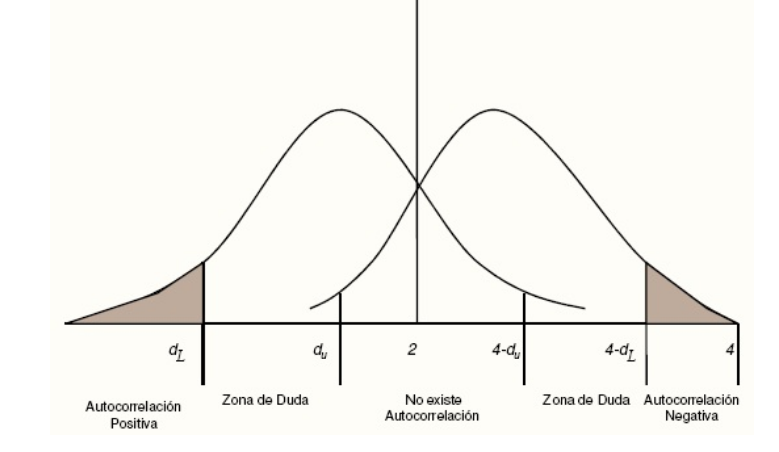
\includegraphics[width=0.7\textwidth]{images/dw.png}
    \caption{Interpretación del estadístico de Durbin-Watson.}
    \label{fig:DW}
\end{figure}

\subsubsection{Reglas de Decisión con el Contraste de Durbin-Watson}

Las tablas estadísticas para el contraste de Durbin-Watson proporcionan dos cotas: una cota inferior ($d_L$) y una cota superior ($d_U$). Las reglas de decisión para evaluar la autocorrelación son las siguientes:

\begin{itemize}
    \item Si $0 < DW < d_L$, se rechaza $H_0$ y se concluye que $\rho > 0$, es decir, existe \textbf{autocorrelación positiva}.
    \item Si $d_L < DW < d_U$, el test es \textbf{no concluyente}.
    \item Si $d_U < DW < 4 - d_U$, se mantiene $H_0$ y se concluye que $\rho = 0$, es decir, los residuos están \textbf{incorrelacionados}.
    \item Si $4 - d_U < DW < 4 - d_L$, el test es \textbf{no concluyente}.
    \item Si $4 - d_L < DW < 4$, se rechaza $H_0$ y se concluye que $\rho < 0$, es decir, existe \textbf{autocorrelación negativa}.
\end{itemize}

Estas reglas permiten interpretar el valor del estadístico $DW$ en función de las cotas obtenidas para el tamaño de muestra y el número de regresores del modelo.


\subsection{Contraste H de Durbin}

El contraste de Durbin-Watson no es válido si en la regresión se incluye algún retardo de la variable dependiente entre las variables explicativas. En este caso, se utiliza el contraste $h$ de Durbin, especialmente en modelos como:

\[
Y_t = \alpha Y_{t-1} + \beta_1 + \beta_2 X_{2t} + \cdots + \beta_k X_{kt} + u_t,
\]
donde $u_t = \rho u_{t-1} + v_t$.

Las hipótesis a contrastar son:

\[
\begin{cases}
H_0 : \rho = 0 & \text{(incorrelación)} \\
H_1 : \rho \neq 0 & \text{(correlación)}
\end{cases}
\]

El estadístico utilizado es:

\[
h = \frac{\rho \cdot \sqrt{n}}{\sqrt{1 - n \cdot \widehat{\text{Var}}(\widehat{\alpha})}} \sim N(0, 1),
\]

donde se rechaza la hipótesis nula si $|h| > Z_{1 - \alpha / 2}$.

\subsection{Contraste de Ljung-Box}

El contraste de Ljung-Box es utilizado para verificar la independencia de los residuos, bajo la hipótesis de que las primeras $m$ autocorrelaciones son iguales a cero. Las hipótesis planteadas son:

\[
\begin{cases}
H_0 : \rho_1 = \rho_2 = \cdots = \rho_m = 0 & \text{(incorrelación)} \\
H_1 : \exists i \in \{1, 2, \dots, m\} \, \text{tal que } \rho_i \neq 0 & \text{(correlación)}
\end{cases}
\]

El estadístico de contraste se define como:

\[
QLB = n(n + 2) \sum_{s=1}^m \frac{r(s)^2}{n - s},
\]

donde $r(s)$ es el coeficiente de autocorrelación muestral de orden $s$:

\[
r(s) = \frac{\sum_{t=s+1}^n e_t e_{t-s}}{\sum_{t=1}^n e_t^2}.
\]

La hipótesis nula se rechaza si:

\[
QLB > \chi^2_{m-1}(1 - \alpha).
\]

Si las observaciones son independientes, los coeficientes $r(s)$ serán cercanos a cero, y no se rechazará la hipótesis nula.

El contraste puede ser implementado en Python utilizando el siguiente comando:

\begin{verbatim}
from statsmodels.stats.diagnostic import acorr_ljungbox
acorr_ljungbox(mco.resid, lags=3)
\end{verbatim}

\subsection{Estimación bajo Autocorrelación}

Consideremos el modelo:

\[
y = X\beta + u,
\]

donde:

\begin{itemize}
    \item $\mathbb{E}[u] = 0$,
    \item $\mathbb{E}[u_i u_j] \neq 0$ para $i \neq j$ con $i, j \in \{1, \dots, n\}$,
    \item $\text{Var}[u] = \sigma^2 \Omega$.
\end{itemize}

Estos supuestos implican que no se cumplen las condiciones de los Mínimos Cuadrados Ordinarios (MCO). Por lo tanto, utilizamos el método de Mínimos Cuadrados Generalizados (MCG), para lo cual necesitamos calcular $P$ tal que $\Omega^{-1} = P^\top P$.

\subsubsection{Modelo Autorregresivo de Orden 1}

Suponemos que $u_t$ sigue un proceso autorregresivo de orden 1, AR(1):

\[
u_t = \rho u_{t-1} + \varepsilon_t,
\]

donde $\varepsilon_t$ es ruido blanco\footnote{El término ruido blanco se refiere a un proceso estocástico con media cero, varianza constante y ausencia de correlación serial.}, $\rho$ es el coeficiente de autocorrelación con $-1 < \rho < 1$.

A partir de esta especificación, se derivan las siguientes relaciones:

\[
\begin{aligned}
    \mathbb{E}[u_t u_{t-1}] &= \rho \sigma^2, \\
    \mathbb{E}[u_t u_{t-2}] &= \rho^2 \sigma^2, \\
    \mathbb{E}[u_t u_{t-3}] &= \rho^3 \sigma^2, \\
    \mathbb{E}[u_t u_{t-k}] &= \rho^k \sigma^2.
\end{aligned}
\]

La matriz de covarianza de $u$, $\Omega$, toma la forma:

\[
\Omega = 
\begin{pmatrix}
1 & \rho & \rho^2 & \cdots & \rho^{n-1} \\
\rho & 1 & \rho & \cdots & \rho^{n-2} \\
\rho^2 & \rho & 1 & \cdots & \rho^{n-3} \\
\vdots & \vdots & \vdots & \ddots & \vdots \\
\rho^{n-1} & \rho^{n-2} & \rho^{n-3} & \cdots & 1
\end{pmatrix}.
\]

Su inversa es:

\[
\Omega^{-1} = \frac{1}{1 - \rho^2}
\begin{pmatrix}
1 & -\rho & 0 & \cdots & 0 \\
-\rho & 1 + \rho^2 & -\rho & \cdots & 0 \\
0 & -\rho & 1 + \rho^2 & \cdots & 0 \\
\vdots & \vdots & \vdots & \ddots & -\rho \\
0 & 0 & 0 & -\rho & 1
\end{pmatrix}.
\]

\subsubsection{Transformación del Modelo}

Partiendo del modelo original:

\[
\begin{aligned}
    y_t &= \beta_1 + \beta_2 X_{2t} + \cdots + \beta_k X_{kt} + u_t, \\
    y_{t-1} &= \beta_1 + \beta_2 X_{2,t-1} + \cdots + \beta_k X_{k,t-1} + u_{t-1},
\end{aligned}
\]

obtenemos la transformación:

\[
y_t - \rho y_{t-1} = \beta_1 (1 - \rho) + \beta_2 (X_{2t} - \rho X_{2,t-1}) + \cdots + \beta_k (X_{kt} - \rho X_{k,t-1}) + (u_t - \rho u_{t-1}).
\]

Definiendo $y_t^* = y_t - \rho y_{t-1}$ y $X_{it}^* = X_{it} - \rho X_{i,t-1}$, el modelo queda:

\[
y_t^* = \beta_1 + \beta_2 X_{2t}^* + \cdots + \beta_k X_{kt}^* + \varepsilon_t,
\]

donde $\varepsilon_t$ cumple los supuestos para aplicar MCO. 

\subsubsection{Primer Observación: Método Prais-Winsten}

Para no perder la primera observación, Prais-Winsten propone:

\[
y_1^* = \sqrt{1 - \rho^2} y_1, \quad X_{i1}^* = \sqrt{1 - \rho^2} X_{i1}.
\]

\subsection{Modificación Prais-Winsten}

El método de Prais-Winsten permite ajustar un modelo con autocorrelación mediante un procedimiento iterativo que combina transformaciones y reestimaciones. El proceso se describe a continuación:

\begin{enumerate}
    \item Estimación inicial por Mínimos Cuadrados Ordinarios (MCO), obteniendo los residuos $e_t$.
    \item Estimación inicial de $\rho$ asumiendo el modelo $u_t = \rho u_{t-1} + \varepsilon_t$, utilizando los residuos $e_t$:
    \[
    \hat{\rho} = \frac{\sum_{t=2}^n e_t e_{t-1}}{\sum_{t=2}^n e_t^2}.
    \]
    \item Transformación del modelo a:
    \[
    y_t^* = y_t - \hat{\rho} y_{t-1}, \quad X_{it}^* = X_{it} - \hat{\rho} X_{i,t-1}.
    \]
    Se estima nuevamente por MCO el modelo transformado:
    \[
    y^* = X^* \beta + u^*,
    \]
    obteniendo nuevos residuos $e_t^*$.
    \item Estimación actualizada de $\rho$ a partir de la regresión $e_t^* = \hat{\rho} e_{t-1}^* + \varepsilon_t^*$:
    \[
    \hat{\hat{\rho}} = \frac{\sum_{t=2}^n e_t^* e_{t-1}^*}{\sum_{t=2}^n (e_t^*)^2}.
    \]
    \item Repetición del proceso: el procedimiento se itera hasta que la estimación de $\rho$ se estabilice, es decir, la diferencia entre iteraciones consecutivas de $\hat{\rho}$ sea menor a $10^{-3}$.
\end{enumerate}

\subsubsection{Proceso Iterativo Cochrane-Orcutt}

El proceso iterativo de Cochrane-Orcutt es similar al de Prais-Winsten, pero omite la primera observación en las transformaciones. Esto simplifica las estimaciones pero puede reducir la eficiencia en muestras pequeñas.

\subsubsection{Implementación en Python}

La implementación del procedimiento iterativo de Prais-Winsten puede realizarse utilizando la clase \texttt{GLSAR} de la biblioteca \texttt{statsmodels}:

\begin{verbatim}
import statsmodels.api as sm

# Ajuste del modelo con iteraciones
model = sm.GLSAR(y, sm.add_constant(x), rho=rho)
results = model.iterative_fit(maxiter=100)
\end{verbatim}

\section{Recursos de Prácticas Relacionados con Python}

Para ello pincha \href{https://github.com/ElblogdeIsmael/ElblogdeIsmael.github.io/tree/main/Asignaturas/Tercer%20A%C3%B1o/ECO/Practicas/Python/econometria-main}{aquí}.

\begin{tcolorbox}[colback=blue!5!white,colframe=blue!75!black, title=Recursos de Prácticas en Econometría con Python]
    \textbf{Nota:} A continuación, se van a ir explicando lo que se considere más relevante de las prácticas de Econometría con Python de cara al examen.
    
\end{tcolorbox}

\subsection{Introducción}


\begin{lstlisting}[style = custompython, caption={Importación de librerías}]
import pandas as pd #librería para manejo de datos


data= pd.read_csv("https://rtgodwin.com/data/houseprice.csv") #Lee base de datos de web...

data
\end{lstlisting}

\begin{lstlisting}[style = custompython, caption={Modelo de Regresión Lineal}]
    import statsmodels.api as sm
    # Modelo Regresión:  modeldata=stock.values
    X=data[["Age", "Rooms"]]
    y=data["Price"]
    
    
    results = sm.OLS(y, sm.add_constant(X)).fit()
    
    print(results.summary())


\end{lstlisting}
\newpage
\subsubsection{Salida}

\begin{verbatim}
    OLS Regression Results                            
==============================================================================
Dep. Variable:                  Price   R-squared:                       0.303
Model:                            OLS   Adj. R-squared:                  0.303
Method:                 Least Squares   F-statistic:                     375.5
Date:                Sat, 04 Jan 2025   Prob (F-statistic):          4.04e-136
Time:                        17:03:06   Log-Likelihood:                -22006.
No. Observations:                1728   AIC:                         4.402e+04
Df Residuals:                    1725   BIC:                         4.404e+04
Df Model:                           2                                         
Covariance Type:            nonrobust                                         
==============================================================================
                 coef    std err          t      P>|t|      [0.025      0.975]
------------------------------------------------------------------------------
const       7.036e+04   6767.987     10.395      0.000    5.71e+04    8.36e+04
Age         -492.3251     67.957     -7.245      0.000    -625.613    -359.037
Rooms       2.206e+04    856.930     25.746      0.000    2.04e+04    2.37e+04
==============================================================================
Omnibus:                      569.117   Durbin-Watson:                   1.572
Prob(Omnibus):                  0.000   Jarque-Bera (JB):             2391.072
Skew:                           1.537   Prob(JB):                         0.00
Kurtosis:                       7.874   Cond. No.                         140.
==============================================================================

Notes:
[1] Standard Errors assume that the covariance matrix of the errors is correctly specified.
\end{verbatim}

\subsubsection{Interpretación de Resultados de la Regresión OLS}

En este análisis, se ajustó un modelo de regresión lineal ordinaria (OLS) para predecir el precio (\textit{Price}) como variable dependiente, utilizando la edad (\textit{Age}) y el número de habitaciones (\textit{Rooms}) como variables explicativas. A continuación, se interpretan los principales resultados:

\begin{itemize}
    \item \textbf{R-cuadrado:} El valor del R-cuadrado es 0.303, lo que indica que el modelo explica aproximadamente el 30.3\% de la variabilidad observada en el precio. Aunque no es un ajuste muy alto, sugiere que las variables incluidas tienen cierta capacidad predictiva.

    \item \textbf{Coeficientes:} 
    \begin{itemize}
        \item El intercepto (\textit{const}) tiene un coeficiente estimado de $7.036 \times 10^4$, lo que implica que, en promedio, cuando las variables explicativas son cero, el precio base es de 70,360 unidades monetarias.
        \item Para la variable \textit{Age}, el coeficiente es de $-492.33$, lo que sugiere que, manteniendo las demás variables constantes, por cada año adicional de antigüedad, el precio disminuye en promedio 492.33 unidades monetarias. Este efecto es estadísticamente significativo ($p < 0.001$).
        \item Para la variable \textit{Rooms}, el coeficiente es de $2.206 \times 10^4$, lo que indica que, manteniendo las demás variables constantes, cada habitación adicional incrementa el precio en promedio 22,060 unidades monetarias. Este efecto también es estadísticamente significativo ($p < 0.001$).
    \end{itemize}

    \item \textbf{Estadísticos de bondad de ajuste y pruebas de diagnóstico:}
    \begin{itemize}
        \item El valor del estadístico de Durbin-Watson es 1.572, lo que sugiere cierta autocorrelación positiva en los residuos.
        \item Las pruebas de normalidad (Omnibus y Jarque-Bera) indican que los residuos no siguen una distribución normal ($p < 0.001$). Esto podría afectar la validez de algunas inferencias estadísticas.
    \end{itemize}

    \item \textbf{Notas:} Los errores estándar asumen que la matriz de covarianzas de los errores está correctamente especificada. La condición de número del modelo es 140, lo que no sugiere problemas graves de multicolinealidad.
\end{itemize}

En resumen, el modelo muestra que la antigüedad afecta negativamente el precio, mientras que el número de habitaciones tiene un impacto positivo y significativo. Sin embargo, la baja capacidad explicativa del modelo y las desviaciones de normalidad en los residuos sugieren que podrían explorarse variables adicionales o transformaciones para mejorar el ajuste.
\newpage

\begin{lstlisting}[style=custompython, caption=Generación de datos sintéticos con numpy]
    # Definimos el número de muestras a generar
    n = 100
    
    # Importamos el paquete numpy para trabajar con arrays y funciones matemáticas
    import numpy as np
    
    # Generamos un array de n valores aleatorios con una distribución normal
    # Media (loc) = 0, Desviación estándar (scale) = 10
    X = np.random.normal(0, 10, n)
    
    # Generamos otra variable Y basada en X, sumándole un ruido aleatorio
    # El ruido se extrae de una distribución normal con media 0 y desviación estándar 1
    Y = X + np.random.normal(0, 1, n)
    \end{lstlisting}
    
    \begin{lstlisting}[style=custompython, caption=Ajuste y visualización de un modelo OLS con statsmodels]
        # Importamos el módulo de visualización matplotlib.pylab
        import matplotlib.pylab as plt
        
        # Graficamos los puntos (X, Y) como un diagrama de dispersión con tamaño de marcador 1
        plt.scatter(X, Y, s=1)
        
        # Mostramos el gráfico
        plt.show()
        
        # Ajustamos un modelo de regresión OLS (Mínimos Cuadrados Ordinarios) a los datos
        results = sm.OLS(Y, sm.add_constant(X)).fit()
        
        # Mostramos un resumen detallado de los resultados del modelo
        results.summary()
        
        # Obtenemos los parámetros estimados: el intercepto (cte) y la pendiente (beta)
        cte = results.params[0]
        beta = results.params[1]
        
        # Graficamos la recta de regresión estimada
        plt.plot([-20, 20], [cte + beta * (-20), cte + beta * 20], color='r')
        
        # Sobreponemos el gráfico de dispersión original
        plt.scatter(X, Y, s=1)
        
        # Mostramos el gráfico con la línea de regresión
        plt.show()
        
        # Importamos herramientas de análisis de estadísticas en statsmodels
        import statsmodels.stats.api as sms
        from statsmodels.compat import lzip
        
        # Cargamos un conjunto de datos de ejemplo sobre crímenes estatales desde statsmodels
        data = sm.datasets.statecrime.load_pandas()
        
        # Accedemos a los datos (endógenos y exógenos)
        data.data
        data.exog
        
        # Definimos y ajustamos un modelo OLS a los datos
        modeloMCO = sm.OLS(data.endog, sm.add_constant(data.exog))
        resultado = modeloMCO.fit()
        
        # Mostramos un resumen de los resultados del modelo
        print(resultado.summary())
        \end{lstlisting}
        
        \begin{figure}[H]
            \centering
            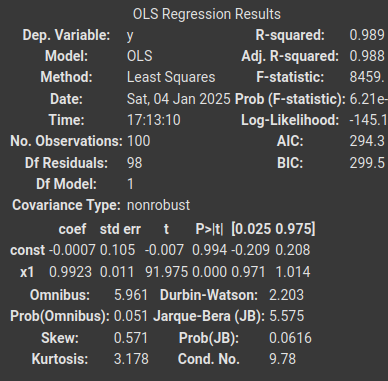
\includegraphics[width=0.7\textwidth]{images/img1.png}
            \caption{Modelo OLS.}
            \label{fig:ols_regression}
        \end{figure}

        \subsubsection{Interpretación de Resultados de la Regresión OLS}

Se ajustó un modelo de regresión lineal ordinaria (\textit{Ordinary Least Squares}, OLS) para explicar la variable dependiente $y$ en función de una única variable independiente $x_1$. A continuación, se presenta el análisis detallado de los resultados:

\begin{itemize}
    \item \textbf{Bondad de ajuste:}
    \begin{itemize}
        \item \textbf{R-cuadrado:} El valor de $R^2$ es 0.989, lo que indica que el modelo explica el 98.9\% de la variabilidad observada en la variable $y$. 
        \item \textbf{R-cuadrado ajustado:} El valor ajustado es 0.988, lo que refleja una ligera penalización por el número de parámetros en el modelo.
    \end{itemize}

    \item \textbf{Coeficientes estimados:}
    \begin{itemize}
        \item El intercepto (\textit{const}) tiene un valor estimado de $-0.0007$, pero no es estadísticamente significativo ($p = 0.994$). Esto implica que el modelo no detecta un impacto relevante de la constante en el valor de $y$.
        \item El coeficiente de la variable $x_1$ es 0.9923, lo que significa que, en promedio, por cada unidad adicional en $x_1$, $y$ aumenta en 0.9923 unidades. Este coeficiente es altamente significativo ($p < 0.001$), con un intervalo de confianza al 95\% que va de 0.971 a 1.014.
    \end{itemize}

    \item \textbf{Estadísticas del modelo:}
    \begin{itemize}
        \item \textbf{Estadístico F:} Con un valor de 8459 y una probabilidad asociada ($p$) de $6.21 \times 10^{-97}$, el modelo tiene una capacidad predictiva altamente significativa.
        \item \textbf{Log-verosimilitud:} El valor de -145.16 es consistente con el ajuste observado.
        \item \textbf{AIC y BIC:} Los valores del Criterio de Información de Akaike (AIC = 294.3) y el Criterio de Información Bayesiano (BIC = 299.5) son útiles para comparar este modelo con otros posibles modelos.
    \end{itemize}

    \item \textbf{Diagnósticos de los residuos:}
    \begin{itemize}
        \item \textbf{Pruebas de normalidad:} La prueba de Omnibus (valor $p = 0.051$) y la prueba de Jarque-Bera (valor $p = 0.0616$) no rechazan la hipótesis de que los residuos siguen una distribución normal al nivel de significancia del 5\%.
        \item \textbf{Durbin-Watson:} El valor de 2.203 sugiere que no hay autocorrelación significativa en los residuos.
        \item \textbf{Condición de número:} Con un valor de 9.78, el modelo no muestra problemas graves de multicolinealidad.
    \end{itemize}
\end{itemize}

En conclusión, el modelo muestra un ajuste excelente, con un coeficiente significativo para $x_1$ que predice el 98.9\% de la variabilidad en $y$. Los diagnósticos no sugieren problemas relevantes en los residuos ni en la especificación del modelo.

\subsubsection{Tipo de Covarianza: nonrobust}

En los resultados del modelo de regresión, la línea \texttt{Covariance Type: nonrobust} indica el tipo de matriz de covarianza utilizado para calcular los errores estándar de los coeficientes estimados. A continuación, se detalla su significado:

\begin{itemize}
    \item \textbf{Nonrobust:} 
    \begin{itemize}
        \item Este tipo de matriz de covarianza supone que los errores (\textit{residuos}) del modelo son \textbf{homocedásticos} (tienen varianza constante) y \textbf{no están correlacionados}.
        \item Bajo esta suposición, los errores estándar, los valores $t$, y los valores $p$ son válidos siempre que se cumplan las condiciones clásicas del modelo de regresión lineal (\textit{Classical Linear Regression Model, CLRM}).
    \end{itemize}
    \item \textbf{Alternativas robustas:} Si las condiciones del CLRM no se cumplen (por ejemplo, si hay heterocedasticidad o autocorrelación en los errores), es posible usar matrices de covarianza ajustadas:
    \begin{itemize}
        \item \textbf{HC0, HC1, HC2, HC3:} Correcciones robustas a la heterocedasticidad, que permiten obtener errores estándar válidos incluso si los residuos tienen varianza no constante.
        \item \textbf{HAC (Heteroskedasticity and Autocorrelation Consistent):} Útil cuando los errores presentan tanto heterocedasticidad como autocorrelación.
    \end{itemize}
\end{itemize}

\textbf{Uso práctico:} En \textit{statsmodels}, se puede especificar un tipo de covarianza robusta al ajustar el modelo, utilizando el argumento \texttt{cov\_type} en el método \texttt{fit}. Por ejemplo:

\begin{lstlisting}[style=custompython, caption=Ajuste de un modelo OLS con covarianza robusta]
results = sm.OLS(Y, sm.add_constant(X)).fit(cov_type='HC3')
\end{lstlisting}

En este caso, se ajustan los errores estándar para ser robustos a la heterocedasticidad.

\textbf{Conclusión:} El uso de \texttt{nonrobust} asume que los residuos cumplen con las condiciones clásicas de homocedasticidad y no autocorrelación. Si estas suposiciones no se verifican, es recomendable optar por una matriz de covarianza robusta para garantizar la validez de las inferencias estadísticas.

\subsection{Autocorrelación}

\begin{lstlisting}[style=custompython, caption=Selección y limpieza de datos en un DataFrame]
    # Seleccionamos las columnas de interés en el DataFrame y eliminamos filas con valores nulos
    datos = datos[['pm2.5', 'TEMP', 'PRES', 'Iws']].dropna()
\end{lstlisting}

\begin{lstlisting}[style=custompython, caption=Cálculo de la estadística de Durbin-Watson para residuos]
    # Importamos la función durbin_watson desde statsmodels
    from statsmodels.stats.stattools import durbin_watson
    
    # Calculamos la estadística de Durbin-Watson sobre los residuos del modelo ajustado
    dw = durbin_watson(mco.resid)
    
    # Imprimimos el resultado de la estadística de Durbin-Watson
    print("Durbin-Watson statistic:", dw)
\end{lstlisting}

\begin{lstlisting}[style=custompython, caption=Detección de autocorrelación con la estadística h de Durbin]
    # Importamos las librerías necesarias
    import numpy as np
    import statsmodels.api as sm
    from statsmodels.stats.stattools import durbin_watson
    
    # Datos simulados: serie autoregresiva
    np.random.seed(0)  # Fijamos la semilla para reproducibilidad
    n = 100  # Número de observaciones
    y_original = datos["pm2.5"]  # Variable original de interés
    y_retardada = np.roll(y_original, 1)  # Variable desplazada una posición hacia atrás
    y_retardada[0] = 0  # Establecemos el primer valor como 0 para evitar problemas
    
    # Ajustamos un modelo OLS con la variable retardada
    modelo = sm.OLS(y_original, sm.add_constant(y_retardada)).fit()
    
    # Extraemos los parámetros del modelo
    beta = modelo.params["x1"]  # Coeficiente estimado para la variable retardada
    var_beta = modelo.bse["x1"] ** 2  # Varianza estimada del coeficiente
    
    # Calculamos la estadística h de Durbin
    h = (1 - dw / 2) * np.sqrt(n / (1 - var_beta))
    
    # Mostramos el valor de h
    print("h-Durbin:", h)
    
    # Verificamos la significancia de h
    if np.abs(h) > 1.96:  # Intervalo de confianza del 95%
        print("Autocorrelación detectada.")
    else:
        print("Autocorrelación no significativa.")
\end{lstlisting}
    
\begin{lstlisting}[style=custompython, caption=Prueba de Ljung-Box para detectar autocorrelación]
    # Importamos la función acorr_ljungbox
    from statsmodels.stats.diagnostic import acorr_ljungbox
    
    # Aplicamos la prueba de Ljung-Box a los residuos del modelo
    # Evaluamos hasta 5 retardos (lags)
    ljungbox_result = acorr_ljungbox(mco.resid, lags=5)
    
    # Mostramos el resultado
    print(ljungbox_result)
\end{lstlisting}

\begin{lstlisting}[language=Python, style=custompython, caption={Implementación de autocorrelación usando GLSAR en Python.}]
    # Calcula el coeficiente rho basado en el estadístico de Durbin-Watson (DW)
    rho = 1 - dw / 2  # dw = 2(1-rho) => rho = 1 - DW/2
    print(rho)  # Imprime el valor calculado de rho
    
    # Ajusta un modelo de regresión generalizada de mínimos cuadrados con autocorrelación (GLSAR)
    mco_autocorr = sm.GLSAR(y, sm.add_constant(X), rho=rho)
    
    # Realiza un ajuste iterativo del modelo hasta un máximo de 100 iteraciones o hasta alcanzar la tolerancia
    res = mco_autocorr.iterative_fit(maxiter=100, rtol=10**(-10))
    
    # Muestra el número de iteraciones realizadas y si el modelo ha convergido
    print('Iteraciones = %d -->  Converge: %s' % (res.iter, res.converged))
    
    # Imprime el valor final de rho utilizado en el modelo
    print('Rho =  ', mco_autocorr.rho)
    
    # Imprime un resumen detallado de los resultados del modelo ajustado
    print(res.summary())
\end{lstlisting}

\begin{lstlisting}[language=Python, style=custompython, caption={Cálculo del Coeficiente de Variación (CV) y prueba de normalidad en los residuos.}]
    # Define una función lambda para calcular el Coeficiente de Variación (CV)
    cv = lambda x: np.std(x, ddof=1) / np.mean(x) * 100
    
    # Aplica la función CV a cada columna del DataFrame 'datos'
    datos.apply(cv)
    
    # Importa el módulo para realizar pruebas estadísticas de Statsmodels
    import statsmodels.stats.diagnostic as diag
    
    # Realiza la prueba de Kolmogorov-Smirnov para verificar la normalidad de los residuos del modelo 'mco'
    diag.kstest_normal(mco.resid)
\end{lstlisting}

\subsection{Práctica 1}

\begin{lstlisting}[language=Python, style=custompython, caption={Conteo de frecuencias para la columna "Fuel.Type" del DataFrame.}]
    # Calcula el conteo de valores únicos en la columna "Fuel.Type" del DataFrame 'datos'
    datos["Fuel.Type"].value_counts()
\end{lstlisting}

\subsection{Test Heterocedasticidad}

\begin{lstlisting}[language=Python, style=custompython, caption={Pruebas de heterocedasticidad y ajuste de mínimos cuadrados ponderados.}]
    # Importa el módulo de diagnóstico estadístico de Statsmodels
    import statsmodels.stats.diagnostic as sm_diagnostic
    
    # GOLDFELD-QUANDT (Prueba para heterocedasticidad en muestras pequeñas)
    # Caso: Hipótesis alternativa de varianza creciente
    GQ = sm_diagnostic.het_goldfeldquandt(y, sm.add_constant(datos["Age"]), alternative="increasing")
    print("Goldfeld Quandt (increasing): ", GQ)
    
    # Caso: Hipótesis alternativa de varianza decreciente
    GQ = sm_diagnostic.het_goldfeldquandt(y, sm.add_constant(datos["Age"]), alternative="decreasing")
    print("Goldfeld Quandt (decreasing): ", GQ)
    
    # Caso: Hipótesis alternativa bilateral
    GQ = sm_diagnostic.het_goldfeldquandt(y, sm.add_constant(datos["Age"]), alternative="two-sided")
    print("Goldfeld Quandt (two-sided): ", GQ)
    
    # BREUSH-PAGAN (Prueba para detectar heterocedasticidad)
    BP = sm_diagnostic.het_breuschpagan(mco.resid, mco.model.exog)
    print("Breush Pagan: ", BP)
    
    # WHITE (Prueba para detectar heterocedasticidad generalizada)
    W = sm_diagnostic.het_white(mco.resid, mco.model.exog)
    print("White: ", W)
    
    # GLEJSER (Prueba para detectar heterocedasticidad con transformación de datos)
    import numpy as np
    z = np.array(datos["Land.Value"].values, dtype=float)
    for h in [-2, -1, -0.5, 0.5, 1, 2]:
        # Ajusta el modelo |e| = delta_0 + delta_1 z^h + eps
        mcoaux = sm.OLS(abs(mco.resid), sm.add_constant(z**h)).fit()
        pval = mcoaux.pvalues["x1"]
        print("h: ", h, "-> pvalt: ", pval, "R2: ", mcoaux.rsquared)
    
    # MÍNIMOS CUADRADOS PONDERADOS (Weighted Least Squares, WLS)
    # Ajusta un modelo ponderando por la raíz cuadrada inversa de z
    mcp = sm.WLS(y, sm.add_constant(X), weights=1. / np.sqrt(z)).fit()
    print(mcp.summary())
\end{lstlisting}

\subsection{Autocorrelación}

\begin{lstlisting}[language=Python, style=custompython, caption={Cálculo del Número de Condición, Factor de Inflación de la Varianza (VIF) y Matriz de Correlaciones.}]
    # IMPORTANTE: El Número de Condición evalúa la colinealidad en el diseño del modelo.
    # Si es alto (típicamente >30 en su forma no raíz cuadrada), indica posible multicolinealidad.
    import numpy as np
    
    # Calcula la raíz cuadrada del Número de Condición del modelo 'mco'
    CN = np.sqrt(mco.condition_number)  # Número de Condición
    print(CN)  # Imprime el Número de Condición para interpretar la estabilidad numérica
    
    # FACTOR DE INFLACIÓN DE LA VARIANZA (VIF)
    # El VIF evalúa la multicolinealidad para cada variable independiente.
    # Valores altos (típicamente >10) indican problemas de multicolinealidad.
    import statsmodels.stats.outliers_influence as oi
    
    # Calcula el VIF para cada variable en el conjunto de predictores 'X'
    vifs = [oi.variance_inflation_factor(X.values, i) for i in range(X.shape[1])]
    vifs  # Devuelve los VIFs calculados para interpretar colinealidad
    
    # MATRIZ DE CORRELACIONES
    # Evalúa la relación lineal entre las variables independientes.
    # Correlaciones altas (>0.8 o <-0.8) pueden sugerir multicolinealidad.
    corr_matrix = np.corrcoef(X.T)  # Calcula la matriz de correlaciones de los predictores
    print(corr_matrix)  # Imprime la matriz para inspeccionar las correlaciones
    
    # VISUALIZACIÓN DE LA MATRIZ DE CORRELACIONES
    # Utiliza gráficos para identificar patrones visuales de multicolinealidad.
    import statsmodels.graphics.api as smg
    import matplotlib.pylab as plt
    
    # Genera un gráfico de correlaciones con nombres de las variables
    smg.plot_corr(corr_matrix, xnames=['Lot.Size', 'Age', 'Land.Value', 'Bedrooms'])
    plt.show()
    \end{lstlisting}

    \subsection{Normalidad}

    \begin{lstlisting}[language=Python, style=custompython, caption={Pruebas estadísticas, estimación de varianza residual, suma de cuadrados y predicción del modelo.}]
        # Prueba de normalidad de Kolmogorov-Smirnov para los residuos
        # Diagnostica si los residuos del modelo siguen una distribución normal.
        # Una p-valor bajo (<0.05) indica que los residuos no son normales.
        import statsmodels.stats.api as sms
        sms.diagnostic.kstest_normal(mco.resid)
        
        # Suma de cuadrados residual (SSR)
        # Representa la variación no explicada por el modelo.
        # Un valor bajo de SSR indica que el modelo ajusta bien los datos.
        mco.ssr
        
        # Estimación de la varianza residual (sigma_gorro)
        # Calcula la varianza de los errores basada en SSR, el número de observaciones (nobs),
        # y el número de parámetros del modelo (params).
        sigmagorro = mco.ssr / (mco.nobs - len(mco.params) - 1)
        sigmagorro
        
        # Suma de cuadrados explicada (ESS)
        # Representa la variación explicada por el modelo. Un valor alto indica que el modelo
        # explica gran parte de la variabilidad de los datos.
        mco.ess
        
        # Predicción del modelo para nuevos datos
        # Estima el valor de la variable dependiente para un conjunto específico de predictores.
        # Ejemplo: [1, 0.009, 0.42, 50000, 90.6, 2] representa los valores de las variables independientes.
        mco.predict([1, 0.009, 0.42, 50000, 90.6, 2])
\end{lstlisting}

\subsection{Anotaciones Extras}

\begin{tcolorbox}[colback=blue!5!white,colframe=blue!75!black, title=Recursos de Prácticas en Econometría con Python]
    \textbf{Nota:} Los que no se hayan mencionado es porque se sobreentiende el código proporcionado anteriormente (Enlace Github).
    
\end{tcolorbox}
        
    
    
    
    
    
        

\end{document}
